\documentclass[utf8]{frontiersSCNS} % for Science, Engineering and Humanities and Social Sciences articles
% \documentclass[utf8]{frontiersFPHY} % for Physics and Applied Mathematics and Statistics articles
\usepackage{gensymb}
\usepackage{url,hyperref,lineno,microtype,subcaption}
\usepackage[onehalfspacing]{setspace}

\usepackage{tabularx}
\linenumbers
\DeclareUnicodeCharacter{0301}{}
\DeclareUnicodeCharacter{2212}{}
\usepackage{wasysym} % provides \DH, \dh, \Thorn, \thorn
% Leave a blank\usepackage{amsmath}
%\DeclareMathOperator{\sign}{sign} line between paragraphs instead of using \\

\usepackage{csvsimple} % for csv tables
\usepackage{booktabs}
\usepackage{multirow}

\def\keyFont{\fontsize{8}{11}\helveticabold }
\def\firstAuthorLast{Balasubramanian {et~al.}} %use et al only if is more than 1 author
\def\Authors{Suryanarayanan Balasubramanian\,$^{1*}$, Martin Hoelzle\,$^{1}$, Michael Lehning\,$^{2}$, Sonam
Wangchuk\,$^{3}$, Johannes Oerlemans\,$^{4}$, Felix Keller\,$^{5,6}$ and Jordi Bolibar\,$^{4}$}
\def\Address{$^{1}$University of Fribourg, Fribourg, Switzerland\\
$^{2}$WSL Institute for Snow and Avalanche Research, Davos, Switzerland\\
$^{3}$Himalayan Institute of Alternatives Ladakh, Leh, India\\
$^{4}$Institute for Marine and Atmospheric Research, Utrecht University, Utrecht, The Netherlands\\
$^{5}$Academia Engiadina, Samedan, Switzerland\\
$^{6}$ETH, Zürich, Switzerland}
\def\corrAuthor{Suryanarayanan Balasubramanian}

\def\corrEmail{suryanarayanan.balasubramanian@unifr.ch}



\begin{document}
\onecolumn
\firstpage{1}

\title[Artificial Ice Reservoirs]{Mass and energy balance calculations for artificial ice reservoirs (Icestupas)}

\author[\firstAuthorLast ]{\Authors}
\address{}
\correspondance{}

\extraAuth{}

\maketitle


\begin{abstract}

Artificial Ice Reservoirs (AIRs) can successfully store water during winter and release the water during spring and
summer. This makes them a reliable fresh water resource for irrigation in dry environments. Several AIRs have been built
but studies of their water storage capacity and efficiency are scarce. This study models a cone-shaped AIR popularly
called Icestupa. Processes involved in the development and temporal evolution of an Icestupa are calculated by a
physically-based model using equations governing the heat transfer, vapour diffusion and transport of water that
undergoes phase changes.  These processes were quantified using meteorological data in conjunction with fountain spray
information (mass input of an AIR) to estimate the quantity of frozen, melted, evaporated and runoff water for three
sites in Switzerland and one in India. At these measurement sites, AIR were built for model
validation purposes. The model was further tested by performing a sensitivity and uncertainty study showing that the
most sensitive parameters are the ice emissivity and the temperature threshold used to determine precipitation phase.
Model calculations estimate that the AIR stored about \% of the total water sprayed as ice. 

\tiny
 \keyFont{ \section{Keywords:} icestupa, mass balance, water storage, climate change adaptation, geoengineering } %All article types: you may provide up to 8 keywords; at least 5 are mandatory.
\end{abstract}

\section{Introduction}

Seasonal snow cover, glaciers and permafrost are expected to change their water storage capacity due to climate change
with major consequences for downriver water supply \citep{Immerzeel_2020}. The challenges brought about by these
changes are especially important for dry mountain environments such as in Central Asia or the Andes, which directly
rely on the seasonal meltwater for their farming and drinking needs \citep{HoelzleBarandun_2019, Apel_2018,
Buytaert_2017, Chen_2016, UNGERSHAYESTEH_2013}. Some villages in Ladakh, India have already been forced to relocate
due to glacial retreat and the corresponding loss of their main fresh water resources \citep{zanskar}. 

\begin{figure} \begin{center} 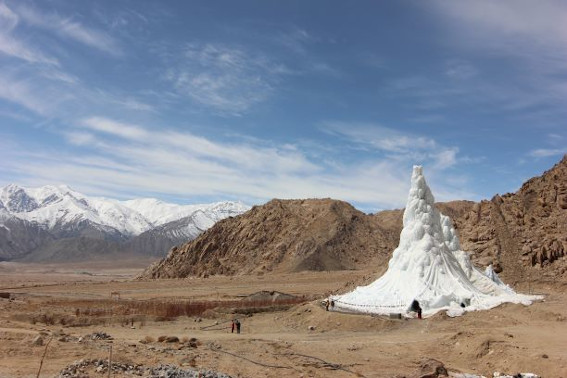
\includegraphics[width=10 cm]{Figures/Figure_1.jpg}
\end{center} \caption{Icestupa in Ladakh, India on March 2017 was 24 $m$ tall and contained around 3700 $m^3$ 
of water. Picture Credits: Lobzang Dadul} \label{fig:cone} \end{figure}

Artificial ice reservoirs (AIRs) have been considered to be a feasible way to adapt to these changes \citep{IPCC_2019,
10.1659/MRD-JOURNAL-D-18-00072.1}. An AIR is a human-made ice structure typically constructed during the cold winter
months and designed to slowly release freshwater during the warm and dry spring and summer months. The main purpose of
AIRs is irrigation. Therefore, AIRs are designed to store water in the form of ice as long into the summer as possible.
The energy required to construct an AIR is usually derived from the gravitational head of the source water body. Some
are constructed horizontally by freezing water using a series of checkdams and others are built vertically by spraying
water through fountain systems \citep{Nusser_2018}. The latter are colloquially referred to as Icestupas and are the
subject of this study.

A typical Icestupa just requires a pipeline attached to a vertically mounted metal pipe with a fountain nozzle for
construction. Their water source is usually a high altitude lake or glacial stream. Due to the altitude difference
between the pipeline input and fountain output, water ejects from the fountain nozzle as droplets that eventually lose
their latent heat to the atmosphere and accumulate as ice around the metal pipe. The fountain nozzle is raised through
addition of further pipes as and when significant ice accumulates. Typically, a dome of branches is constructed around
the metal pipe so that such pipe extensions can be done from within this dome. During the winter, the fountain is
manually activated from sunset to sunrise. Threads, tree branches and fishing nets are used to guide and accelerate the
ice formation.

Since their invention in 2013 \citep{campaign}, Icestupas have gained widespread publicity in the region of Ladakh,
Northern India since they require very little infrastructure, skills and energy to be constructed in comparison to
other water storage technologies. Compared to other AIR geometries, Icestupas (Fig. \ref{fig:cone}) can be built at
lower altitudes and last much longer into the summer than other types of ice structures \citep{campaign}. However, to
date, no reliable estimates exist about the amount of sprayed water that is necessary to create them and the meltwater
they provide \citep{Nusser_2018}. Rough estimates of Icestupa meltwater in Ladakh suggest that the water loss during
the construction process is considerable (see Appendix \ref{section:ladakhloss}). A complete set of measurements of the
water storage and energy balance are required to understand the cause of the water losses better and increase the
construction efficiency.
 
In this paper, we aim to develop a physically-based model of a vertical AIR (or Icestupa) that can quantify their
storage efficiency using existing weather and water usage information. Mass and energy balance equations were used to
estimate the quantity of water frozen, melted, evaporated and runoff. Sensitivity and uncertainty analysis were
performed to identify the most critical parameters and the variance caused by them. For validation, we chose four AIR
built across the winters of 2019, 2020 and 2021 in India and Switzerland.Our model and validation experiments provide
first steps towards evaluating the effectiveness of a vertical AIR for irrigation and allow us to outline some
preliminary guidelines for consideration when a construction of an Icestupa for water storage is envisaged. 

\section{Study Sites}
To accurately calibrate, estimate and validate the ice volume of AIR the model requires three kinds of measurements namely, weather,
water and ice volume. So through the winters of 2019, 2020 and 2021 several scientific AIR were constructed by teams in
Switzerland and India. Here we present the results of three scientific AIR which have a relatively complete dataset
associated with them as shown in Table \ref{tab:3AIR}. 


\subsection{Measurement sites}

The Guttannen (CH21) site in the Bern region lies at 1047 $m$ a.s.l.. In the winter (Oct-Apr), mean daily minimum and
maximum air temperatures vary between -13 and 15 $\degree C$. Clear skies are rare, averaging around 7 days during
winter \citep{eispalast}. The site was situated adjacent to a stream resulting in high humidity values across the study
period as shown in Fig. \ref{fig:CH21site}. The fountain used for spraying water had an initial height of 2.3\,$m$. The
water was transferred from a spring water source and flowed via a flowmeter to the nozzle.  In addition, a webcam
guaranteed a continuous survey of the site during the construction of the AIR.

\begin{figure} 
    \begin{center} 
        \includegraphics[width=10 cm]{Figures/DJI_0161.jpg} 
    \end{center} 
\caption{Bird's eye view of the CH21 AIR} 
\label{fig:CH21site} 
\end{figure}


The CH21 AIR was constructed by Guttannen Bewegt Association on a garden adjacent to a stream in Guttannen, Switzerland.
To initiate the ice formation process, tree branches were laid covering the fountain pipe.  The fountain height varied
between 2 to 5\,$m$ during the construction period. Fountain operation was guided by temperature conditions. 

The Gangles(IN21) site in the Ladakh region lies at 4025 $m$ a.s.l..

\subsection{Weather measurements} 
Air temperature, relative humidity, wind speed, pressure, longwave, shortwave direct and diffuse radiation are required
to calculate the surface energy balance of an AIR. 

For the CH site, the primary weather data source was a meteoswiss AWS located 184 m away. In addition, we used ERA5
reanalysis dataset \citep{era5} for filling data gaps and adding data that were not measured directly as shown in Fig.
\ref{fig:input}. Zero wind speed values were recorded whenever snow accumulated on the ultrasonic wind sensor. It was
assumed this was the cause when null wind speeds were observed continuously for atleast 3 hours. All such null values
were replaced using the ERA5 dataset. 

The ERA5 reanalysis dataset has a good correlation with lower elevation sites in Switzerland
\citep{Scherrer_2020}. The ERA5 grid point chosen (Latitude 46° 38' 24" N, Longitude 8° 15' 00" E) for the CH21 site was
around 3.6 km away from the actual site.  All the ERA5 variables were therefore fitted with the meteoswiss dataset via
linear regressions.

For the IN site, the primary weather data source was a campbell weather station located adjacent to the AIR. In
addition, we used another campbell AWS located 12 km away for filling data gaps and adding data that were not measured
directly as shown in Fig. \ref{fig:input}.

\begin{figure} 
    \centering 
    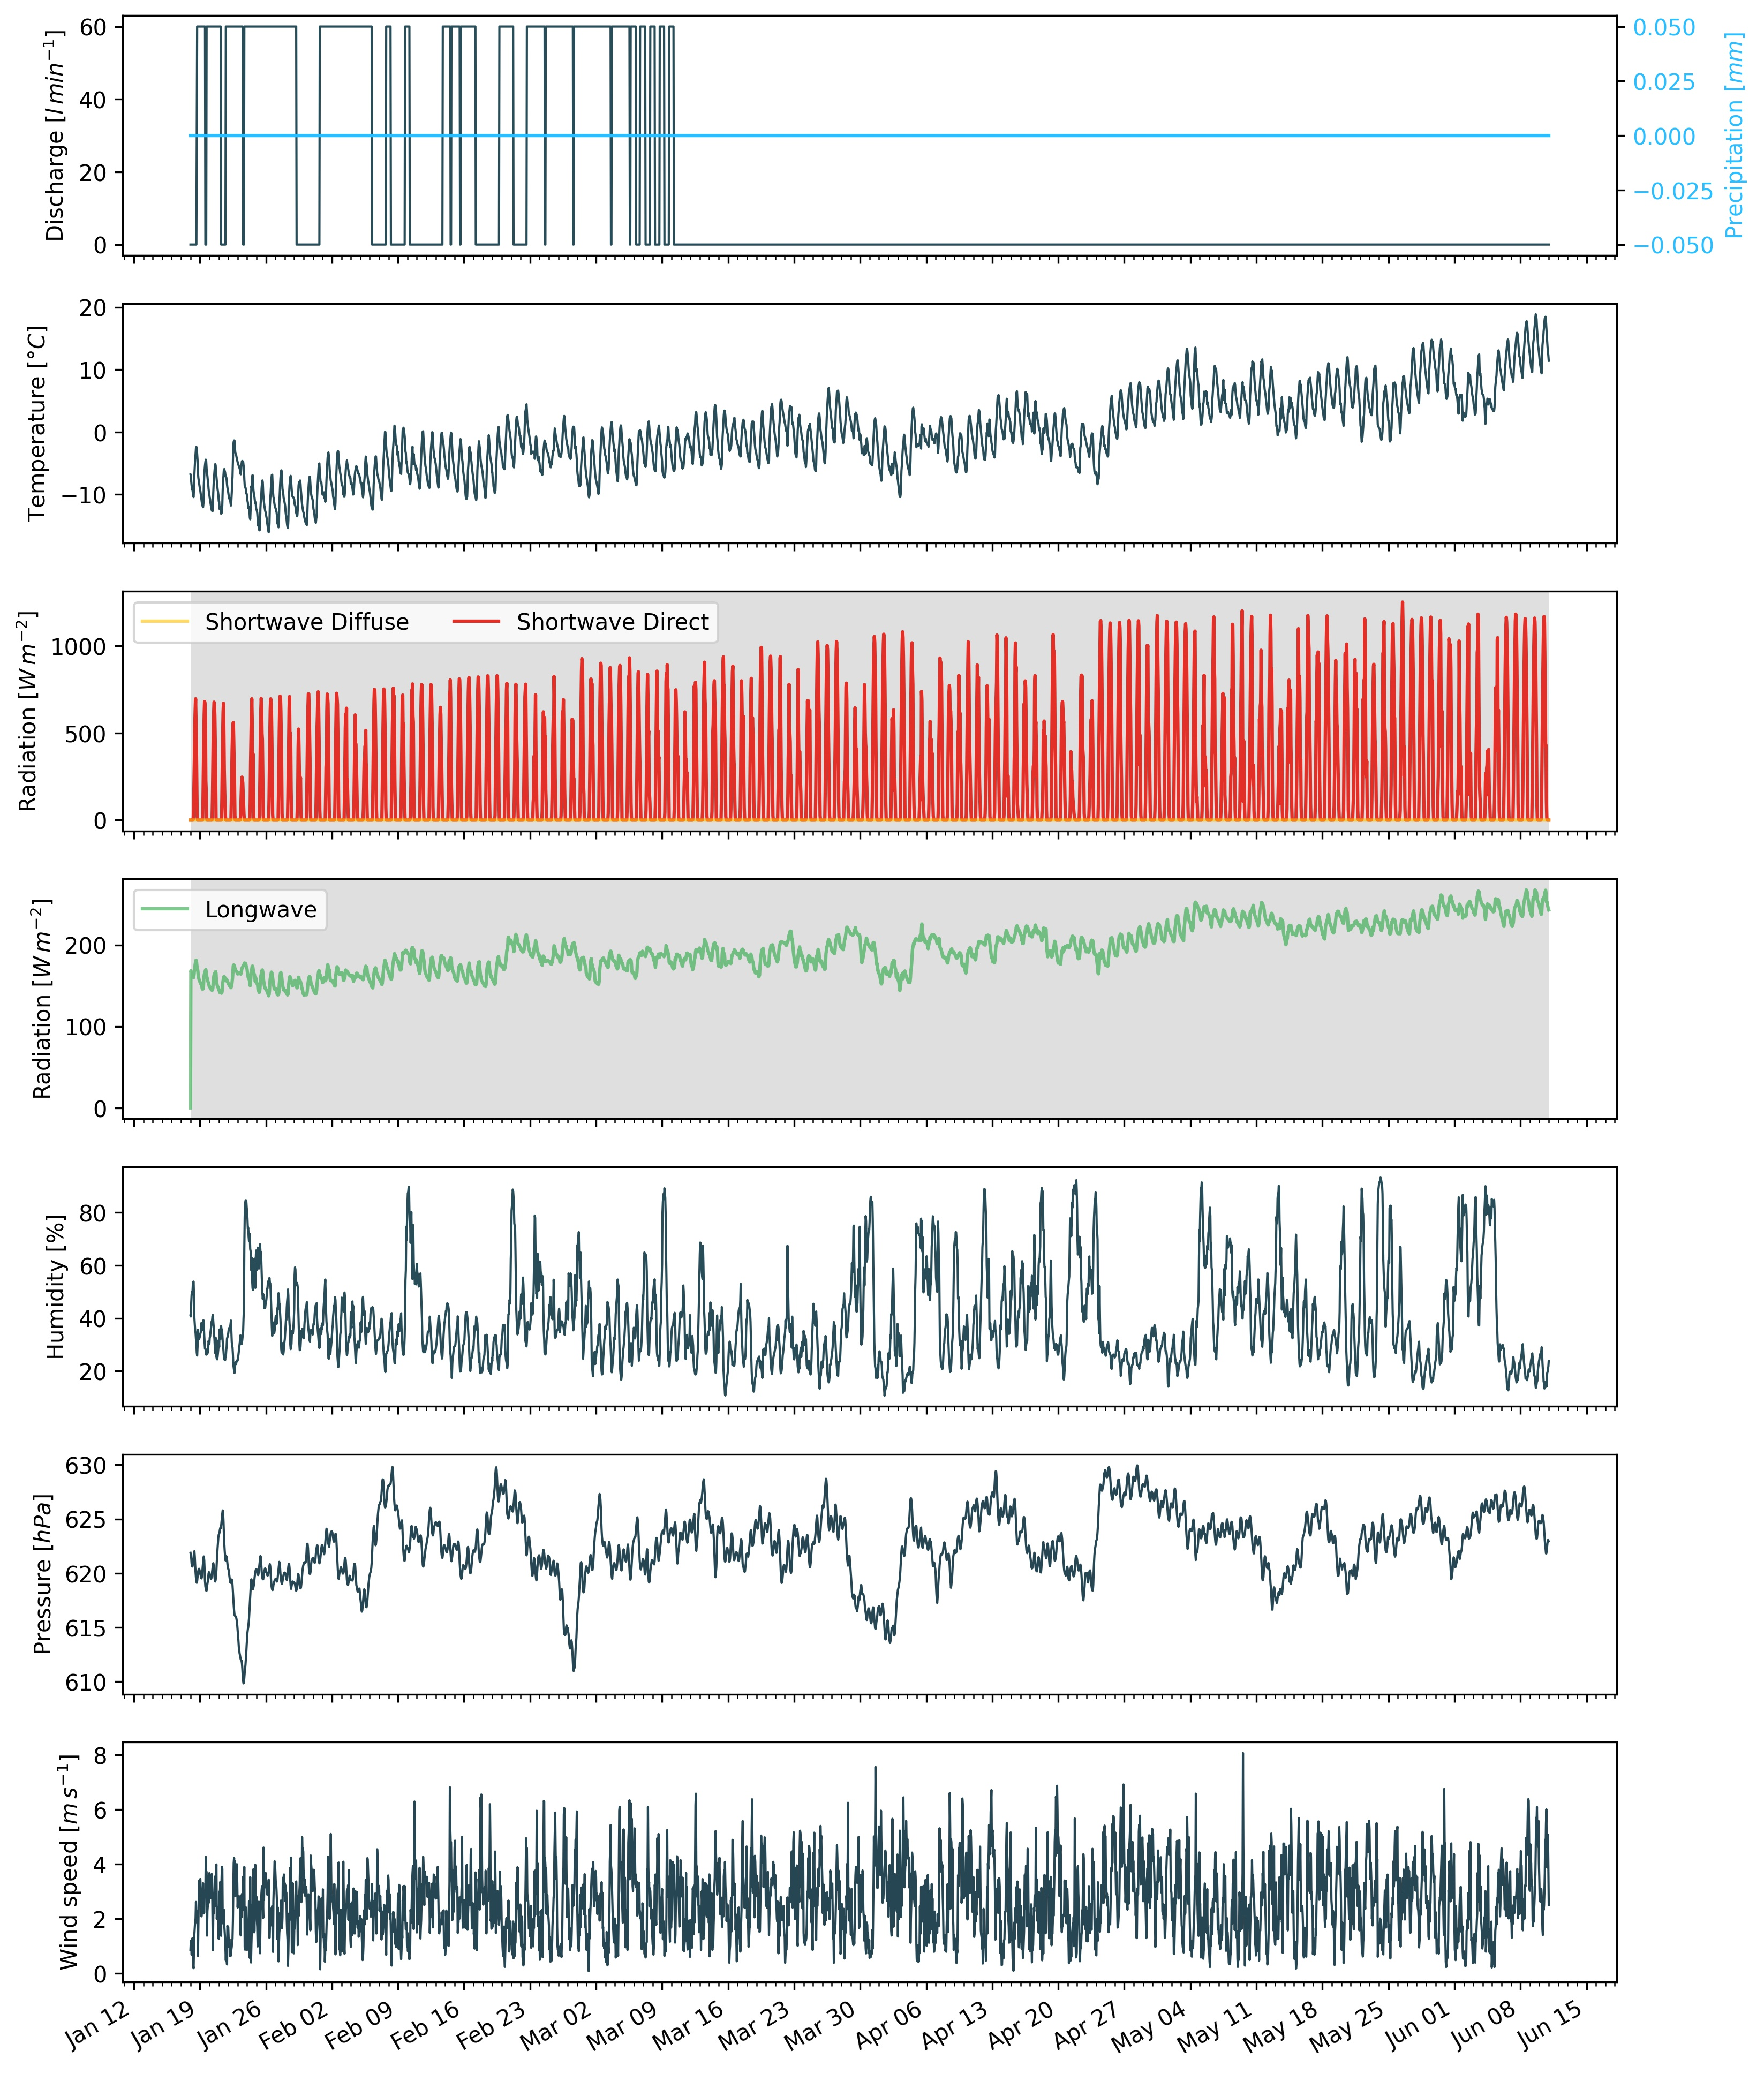
\includegraphics[width=\linewidth]{./Figures/Model_Input.jpg} 
\caption{Measurements at the AWS of CH21 were used as main model input data in hourly frequency. Missing data, data gaps
and errors were filled from the ERA5 dataset (shaded regions).} 
    \label{fig:input} 
\end{figure}

\subsection{Discharge measurements} 
The water flow rate or discharge was measured via an ultrasonic sensor attached to the fountain supply pipeline.
However, due to various malfunctions, the discharge measurements were very sparse and could not be extrapolated for the
complete measurement period for both the CH and In site. Instead the discharge duration was first determined and then
the available discharge measurement was used to determine the average discharge quantity $d_{mean}$ during these
periods. 

For the CH site, the fountain was never switched off so the discharge duration was extrapolated from just from one
fountain on and off event each. The discharge quantity during this duration varied as shown by the sparse flowmeter
measurements captured. Here we assume a constant discharge quantity $d_{mean}$ calculated from the mean of the available
flowmeter measurements. 

For the IN site, even though the fountain was never manually switched off, there were many pipeline freezing events that
interrupted the discharge duration. So discharge rate was extrapolated to be the mean discharge $d_{mean}$ except during
these pipeline freezing events.

\subsection{Ice volume measurements}
Several Drone flights were conducted in the CH and IN sites. The DEM generated through these flights were analysed to obtain
the circumference and volume of the ice structure. The mean circumference measured during the fountain duration was set
as the spray radius ($r_{spray}$) and the first drone flight was used to set the dome volume ($V_{dome}$) for model
initialisation. The ice volume data was later used for calibration and validation of the model. 
 
\begin{table}[h]
\centering
\caption{The Scientific AIR }
\label{tab:3AIR}
\begin{tabular}{@{}|l|l|l|l|@{}}
\toprule
\textbf{AIR}      & \textbf{Gangles, 2021} & \textbf{Guttannen, 2021} & \textbf{Guttannen, 2020} \\ \midrule
Shortname                      & IN21 & CH21 & CH20 \\ \midrule
Altitude {[}$m$ a.s.l.{]} & 4025 & 1047 & 1047 \\ \midrule
Fountain Duration & Jan 18 - Mar 10        & Nov 22 - Feb 20          & Jan 3 - Mar 8\\ \midrule
Drone Flights             & 6    & 9    & 3      \\ \midrule
$r_{spray}$ {[}$m${]}     & 10.8 & 6.9  & 7.7   \\ \midrule
$V_{dome}$ {[}$m^{3}${]}  & 78.5 & 13.2 & 23.9  \\ \midrule
$d_{mean}$ {[}$l/min${]}  & 60 & 7.5 & 7.5  \\ \bottomrule
\end{tabular}
\end{table}

\section{Model setup}

A bulk energy and mass balance model is used to calculate the amounts of ice, meltwater, water vapour and runoff water
of the AIR every hour. This model consists of four modules which estimates the AIR, a) geometric evolution , b) energy
balance, c) surface temperature and d) mass balance. 

  \begin{figure} \begin{center} 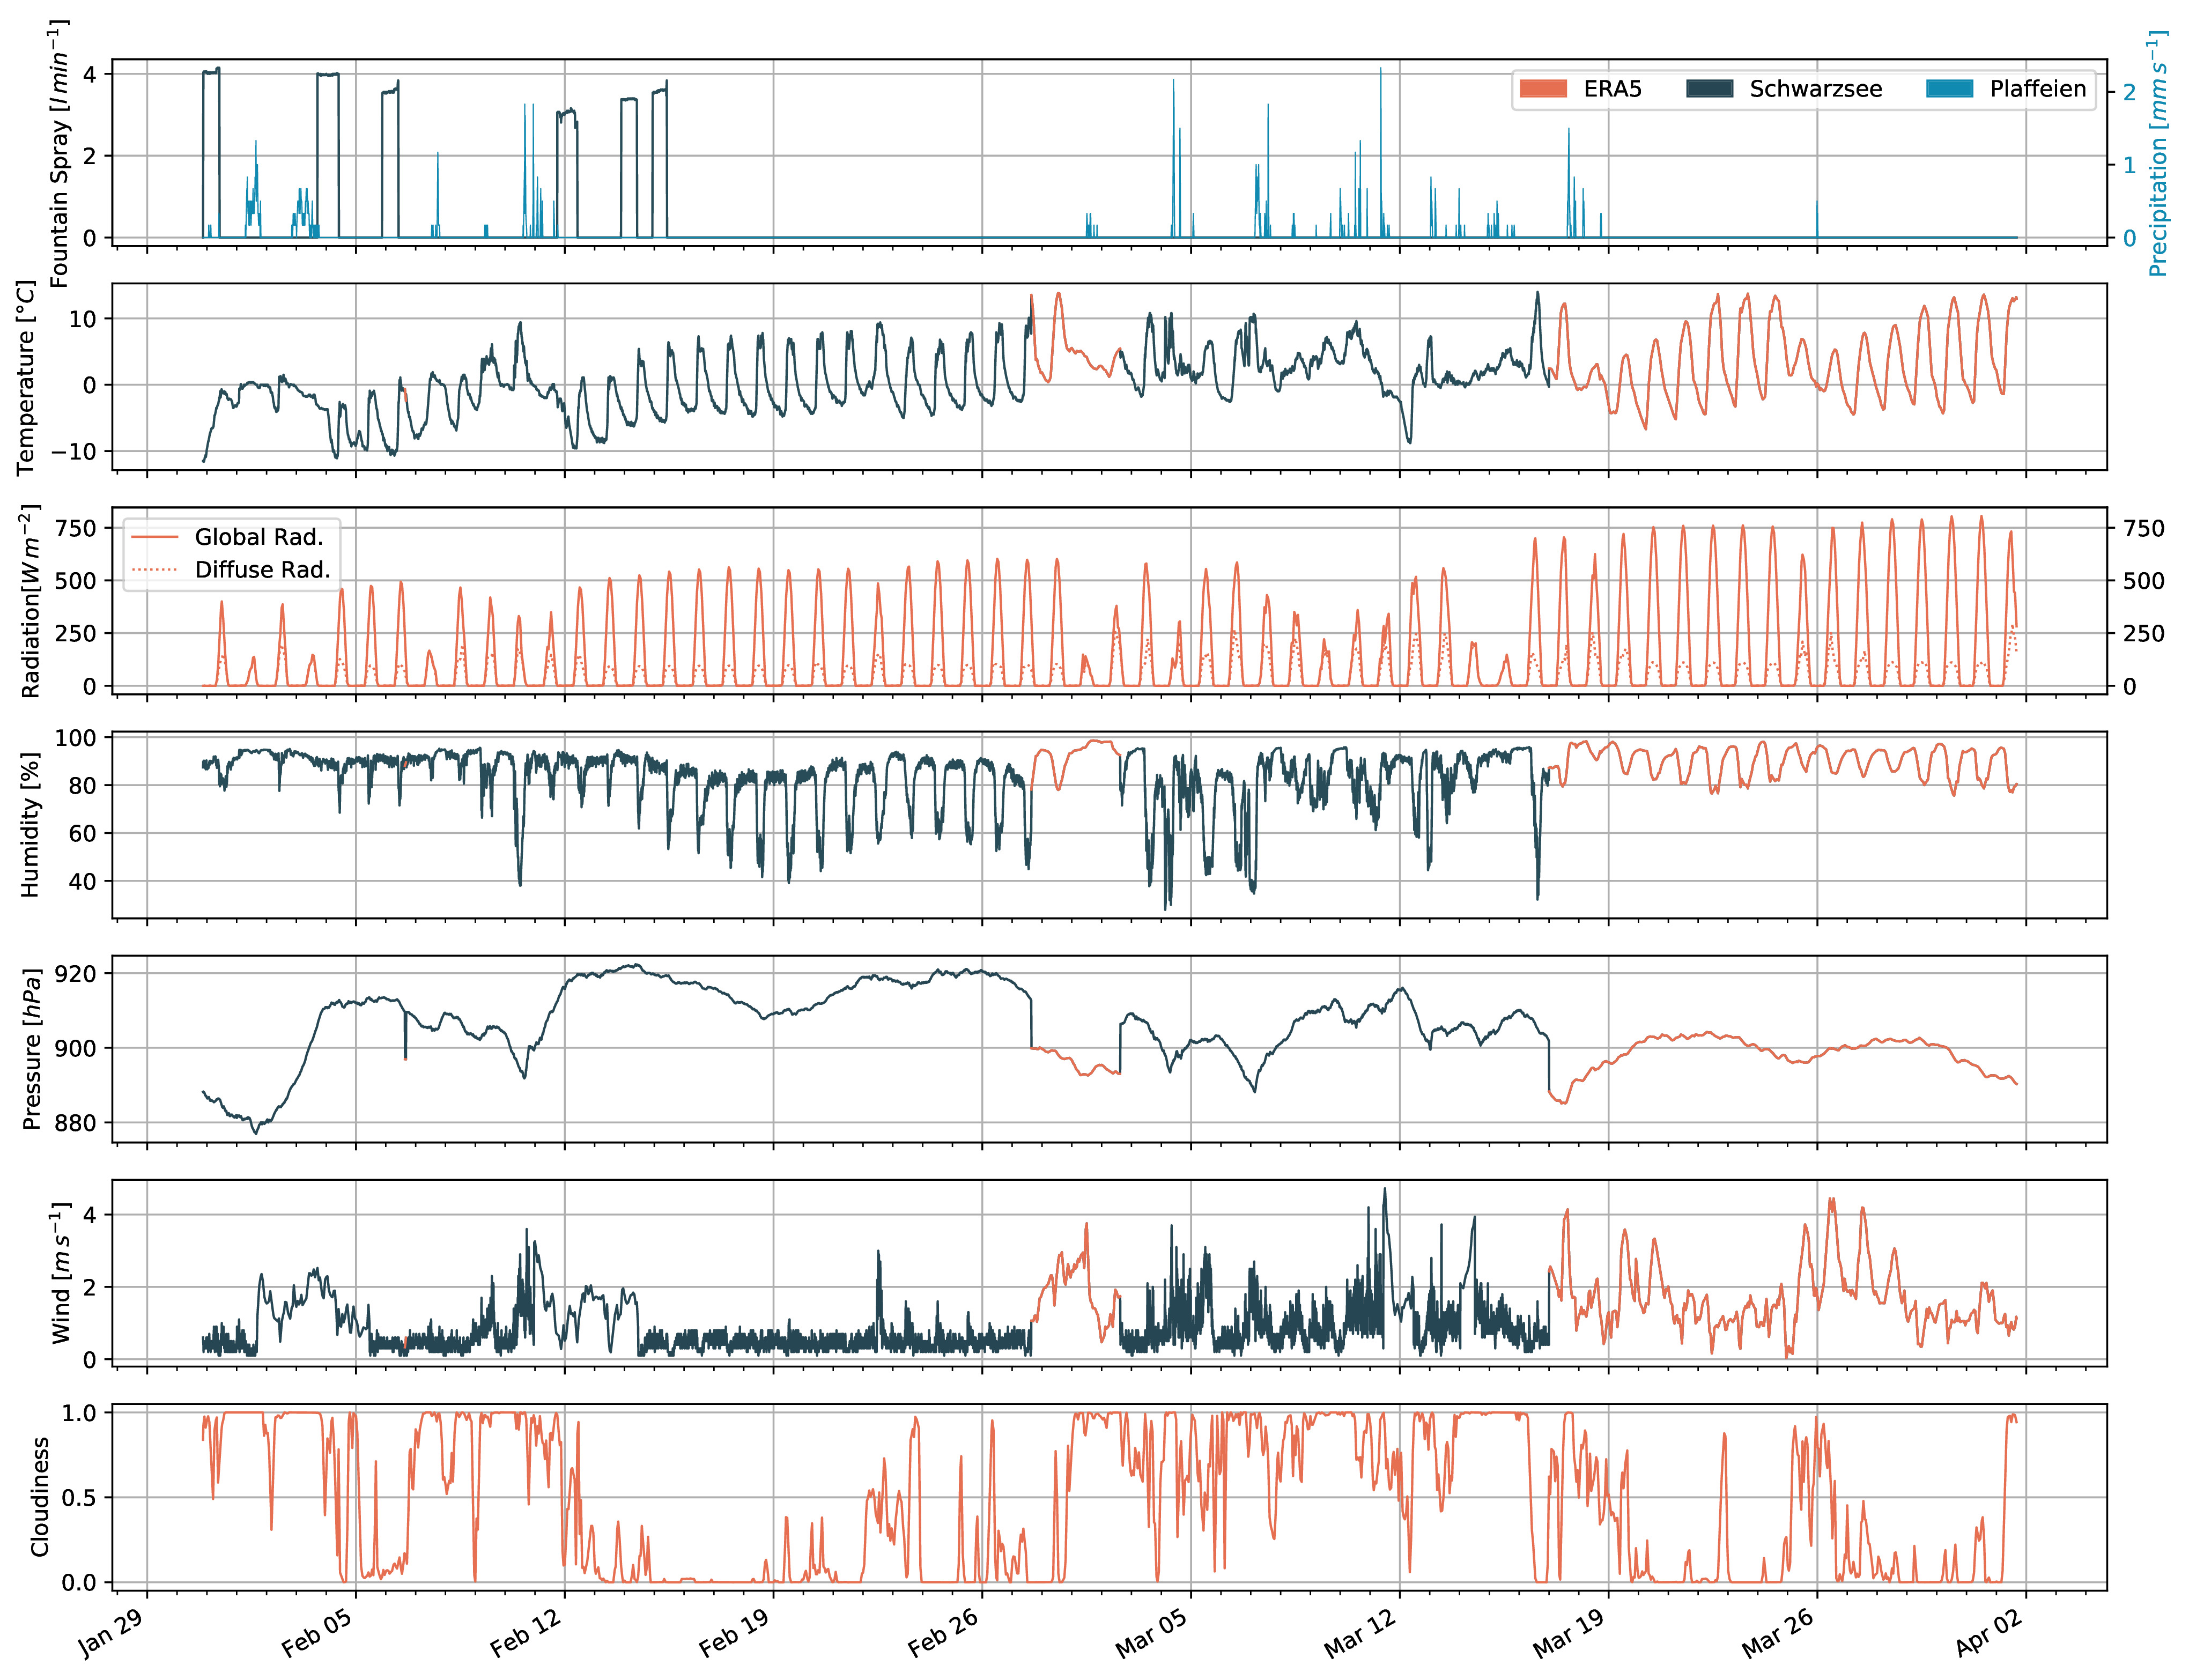
\includegraphics[width=15 cm]{Figures/Figure_4.jpg} \end{center} \caption{Model
schematic showing the algorithm used in the model at every time step. Further details about the variables can be
found in the associated tables and figures.} \label{fig:schema} \end{figure}

\subsection{Geometric evolution}

Radius $r_{ice}^i$ and height $h_{ice}^i$ define the dimensions of the AIR assuming its geometry to be a cone. The
surface area $A^i$ exposed to the atmosphere and volume $V^i$ are:

\begin{equation} A = \pi \cdot r_{ice} \cdot \sqrt{{r_{ice}}^2 + {h_{ice}}^ 2} \label{eqn:A} \end{equation}

\begin{equation} V = \pi/3 \cdot {r_{ice}}^2 \cdot h_{ice} \label{eqn:V} \end{equation}

Note that we do not specify the time step superscript $i$ of the shape variables $A$, $V$, $r_{ice}$ and $h_{ice}$ for
brevity.  The equations used henceforth display model time step superscript $i$ only if it is different from the
current time step.

With the mass of the AIR $M_{ice}$, its current volume can also be expressed as: 

\begin{equation} V = M_{ice} /\rho_{ice} \label{eqn:V1} \end{equation} 

where $\rho_{ice}$ is the density of ice (917 $kg\, m^{-3}$). 


The influence of the AIR fountain is parameterised by the fountain water temperature $T_{w}$ and its spray radius $r_{spray}$.
The initial radius $r_0$ of the AIR is assumed to be $r_{spray}$. The initial height $h_0$ depends on the dome volume
$V_{dome}$ used to construct the AIR as follows:

\begin{equation} 
    h_{0} =  \Delta x + \frac{3 \cdot V_{dome}}{\pi r_{spray}^2 } 
\label{eqn:h0}
  \end{equation}

where $\Delta x$ is the surface layer thickness (defined in Section \ref{section:EB})

During subsequent time steps, the dimensions of the AIR evolve assuming a uniform ice formation and decay across
its surface area with an invariant slope $s_{cone} = \frac{h_{ice}}{r_{ice}}$ .  During
these time steps, the volume is parameterised using Eqn. \ref{eqn:V} as:\begin{equation} V = \frac{\pi \cdot {r_{ice}}^3
    \cdot s_{cone}}{3} \label{eqn:V2} \end{equation} 


However, the Icestupa cannot outgrow the maximum range of the water droplets ($(r_{ice})_{max} = r_{F}$). Combining
equations \ref{eqn:V}, \ref{eqn:h0}, \ref{eqn:V1} and \ref{eqn:V2}, the geometric evolution of the Icestupa at each time step $i$ can
be determined by considering the following rules:

\begin{equation} (r_{ice},\, h_{ice}) = \left\{ \begin{array}{ll} (r_{spray} ,\, h_0) & \textit{ if } i=0\\
    (r_{ice}^{i-1},\, \frac{3 \cdot M_{ice}}{\pi \cdot \rho_{ice} \cdot {(r_{ice}^{i-1})}^2}) & \textit{ if }
    r_{ice}^{i-1} \geq r_{F} \textit{ and } \Delta M_{ice} > 0 \\ (\frac{3 \cdot M_{ice}}{\pi \cdot \rho_{ice} \cdot s_{cone}})^{1/3} \cdot (1,\,  s_{cone}) &
otherwise \end{array} \right.  \label{eqn:A2} \end{equation}

where $\Delta M_{ice} = M_{ice}^{i-1} - M_{ice}^{i-2}$

    \begin{figure} \begin{center} 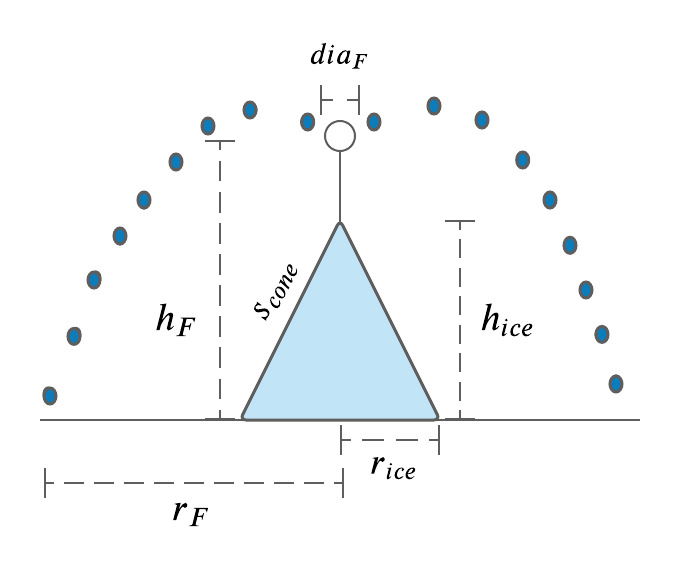
\includegraphics[width=10
cm]{Figures/Figure_5.jpg} \end{center} \caption{Shape variables and fountain constants of the CH21 Icestupa. $r_{ice}$ is
the radius, $h_{ice}$ is the height and $s_{cone}$ is the slope of the ice cone. $r_{spray}$ is the spray radius, $h_F$ is the
height and $dia_F$ is the nozzle diameter of the fountain.} \label{fig:shape} \end{figure}

\subsection{Energy Balance} \label{section:EB}

The energy balance equation \citep{Hock_2005} for the AIR is formulated as follows:

\begin{equation} q_{SW} + q_{LW} + q_{L} + q_{S} + q_{F} + q_{G} = q_{surf} \label{eqn:EB} \end{equation}

where $q_{surf}$ is the surface energy flux in [$W\,m^{-2}$]; $q_{SW}$ is the net shortwave radiation; $q_{LW}$ is the
net longwave radiation; $q_{L}$ and $q_{S}$ are the turbulent latent and sensible heat fluxes. $q_{F}$ represents the heat
exchange of the fountain water droplets with the AIR ice surface. $q_{G}$ represents ground heat flux between Icestupa
surface and Icestupa interior. Energy transferred in the direction of the ice surface is always denoted as positive and
away as negative.  

% TODO Introduce surface layer rate
Equation \ref{eqn:EB} is usually referred to as the energy budget for “the surface”, but practically it must apply to
a surface layer of ice with a finite thickness $\Delta x$. The energy flux acts upon the Icestupa surface layer which
has an upper and a lower boundary defined by the atmosphere and the ice body of the Icestupa, respectively. The
parameter selection for $\Delta x$ is based on the following two arguments: (a) the ice thickness $\Delta x$ should be
small enough to represent the surface temperature variations every model time step $\Delta t$ and (b) $\Delta x$ should
be large enough for these temperature variations to not reach the bottom of the surface layer.  Therefore, we introduced
a 20 $mm$ thick surface layer for a model time step of 1 hour, over which the energy balance is calculated. A
sensitivity analysis was later performed to understand the influence of this factor. Here, we define the surface
temperature $T_{ice}$ to be the modelled average temperature of the Icestupa surface layer and the energy flux $q_{surf}$
is assumed to act uniformly across the Icestupa area $A$.

\subsubsection{Net Shortwave Radiation \texorpdfstring{$q_{SW}$}{Lg}} 
The net shortwave radiation $q_{SW}$ is computed as follows:
\begin{equation} q_{SW} = (1- \alpha)\cdot (SW_{direct} \cdot f_{cone} + SW_{diffuse}) \label{eqn:SW} \end{equation}

where $SW_{direct}$ and $SW_{diffuse}$ are the ERA5 direct and diffuse short wave radiation, $\alpha$ is the modelled
albedo and $f_{cone}$ is the area fraction of the ice structure exposed to the direct shortwave radiation.

We model the albedo using a scheme described in \cite{OerlemansKnap_1998}. The scheme records the decay of albedo with
time after fresh snow is deposited on the surface. $\delta t$ records the number of time steps after the last snowfall
event. After snowfall, albedo changes over a time step, $\delta t$ , as

\begin{equation} \alpha=\alpha_{ice}+(\alpha_{snow}-\alpha_{ice}) \cdot e^{(-\delta t)/\tau} \label{eqn:a}
\end{equation}

where $\alpha_{ice}$ is the bare ice albedo value (0.35), $\alpha_{snow}$ is the snow ice albedo value (0.85) and
$\tau$ is a decay rate, which determines how fast the albedo of the ageing snow reaches this value.  The decay rate
$\tau$ is assumed to have a base value of 10 days similar to values obtained by \cite{Schmidt_2017} for wet surfaces
and its maximal value is set based on observations by \cite{OerlemansKnap_1998} as shown in Table
\ref{tab:parameters}.  Furthermore, the albedo $\alpha$ varies depending on the water source that formed the current
Icestupa surface.  Correspondingly, the albedo is reset to the value of bare ice albedo if the fountain is spraying
water onto the current ice surface and to the value of fresh snow albedo if a snowfall event occurred. Snowfall events
are assumed if the air temperature is below $T_{ppt}=1 \degree C$ \citep{FujitaAgeta_2000}.

The area fraction $f_{cone}$ of the ice structure exposed to the direct shortwave radiation depends on the shape
considered. The direct solar radiation incident on the AIR surface is first decomposed into horizontal and vertical
components using the solar elevation angle $\theta_{sun}$. For a conical shape, half of the total curved surface is
exposed to the vertical component of the direct shortwave radiation and the projected triangle of the curved surface is
exposed to the horizontal component of the direct shortwave radiation. The solar elevation angle $\theta_{sun}$ used is
modelled using the parametrisation proposed by \cite{Woolf_1968}. Accordingly, $f_{cone}$ is determined as follows:

\begin{equation} \begin{split} f_{cone}& =\frac{(0.5 \cdot r_{ice} \cdot h_{ice}) \cdot cos \theta_{sun} +(\pi \cdot
{r_{ice}}^2/2) \cdot sin \theta_{sun} }{\pi \cdot r_{ice} \cdot ({r_{ice}}^2+{h_{ice}}^2)^{1/2}}\\ \end{split}
\label{eqn:f_{cone}} \end{equation}

The ERA5 diffuse shortwave radiation is assumed to impact the conical Icestupa surface uniformly. 

\subsubsection{Net Longwave Radiation \texorpdfstring{$q_{LW}$}{Lg}}

The net longwave radiation $q_{LW}$ is determined as follows:

\begin{equation} q_{LW}= LW_{in}-\sigma \cdot \epsilon_{ice} \cdot {(T_{ice}+ 273.15)}^4
\label{eqn:LW} \end{equation}

where $T_a$ represents the measured air temperature, $T_{ice}$ is the modelled surface temperature, both temperatures
are given in [$\degree C$], $\sigma=5.67\cdot 10^{-8}\,Jm^{-2}s^{-1}K^{-4}$ is the Stefan-Boltzmann constant, $LW_{in}$
denotes the incoming longwave radiation derived from the ERA5 dataset and $\epsilon_{ice}$ is the corresponding
emissivity value for the Icestupa surface (see Table \ref{tab:parameters}).

\subsubsection{Turbulent sensible \texorpdfstring{$q_{S}$}{Lg} and latent \texorpdfstring{$q_{L}$}{Lg} heat fluxes }

The turbulent sensible $q_{S}$ and latent heat $q_{L}$ fluxes are computed with the following expressions proposed by
\cite{Garratt_1992}:

\begin{equation} q_{S}=c_{a} \cdot \rho_{a} \cdot p_{a}/p_{0,a} \cdot \frac{\kappa^2 \cdot v_a \cdot
(T_a-T_{ice})}{{(\ln{\frac{h_{AWS}}{z_{ice}}})}^2} \label{eqn:qs} \end{equation}

\begin{equation} q_{L}=0.623 \cdot L_s \cdot \rho_{a}/p_{0,a} \cdot \frac{\kappa^2 \cdot
v_a(p_{v,a}-p_{v,ice})}{{(\ln{\frac{h_{AWS}}{z_{ice}}})}^2} \end{equation}

where $h_{AWS}$ is the measurement height above the ground surface of the AWS (in $m$), $v_a$ is the wind speed in
[$m\,s^{-1}$], $c_a$ is the specific heat of air at constant pressure (1010 J $kg^{-1} K^{-1}$), $\rho_{a}$ is the air
density at standard sea level (1.29 $kg m^{-3}$), $p_{0,a}$ is the air pressure at standard sea level (1013 $hPa$),
$\kappa$ is the von Karman constant (0.4), $L_s$ is the heat of sublimation (2848 $kJ\, kg^{-1}$) and $z_{ice}$ (1.7
$mm$) denotes the roughness length of ice (momentum and scalar).  The vapor pressures over air ($p_{v,a}$) and ice
($p_{v,ice}$) was obtained using the following formulation given in \cite{WMO_2018}:

\begin{equation} \begin{split} p_{v,a}&=6.107 \cdot 10^{(7.5 \cdot T_a / (T_a + 237.3))}\\ p_{v,ice}&=(1.0016 +
3.15\cdot10^{-6}\cdot p_{a}-0.074\cdot p_{a}^{-1})\cdot(6.112 \cdot e^{(22.46 \cdot T_{ice} / (T_{ice} + 272.62))})
\end{split} \label{eqn:vp} \end{equation}

where $p_{a}$ is the measured air pressure in [$hPa$].  

\subsubsection{Fountain water heat flux \texorpdfstring{$q_{F}$}{Lg} }

The interaction between the fountain water and the ice surface is taken into account by assuming that the ice surface
temperature remains constant at 0 $\degree C$ during time steps when the fountain is active. This process can be divided
into two simultaneous steps: (a) the water temperature $T_{water}$ is cooled to 0 $\degree C$ and (b) the ice surface
temperature is warmed to 0 $\degree C$. Thus, the heat flux caused by the fountain water is calculated as follows:

\begin{equation} 
  q_{F} = \left\{ \begin{array}{ll}
         0 & \textit{ if } \Delta M_{F} = 0\\ \frac{ \Delta M_F \cdot c_{water} \cdot T_{water}}{\Delta t \cdot A} +
         \frac{\rho_{ice} \cdot \Delta x \cdot c_{ice} \cdot T_{ice}}{\Delta t} & \textit{ if } \Delta M_{F} > 0 
    \end{array} \right.  \label{eqn:qF}
\end{equation} 
with $c_{ice}$ as the specific heat of ice. 

\subsubsection{Bulk Icestupa heat flux \texorpdfstring{$q_{G}$}{Lg}} \label{sec:Bulkflux}
% TODO Reason choice of lice
The bulk Icestupa heat flux $q_{G}$ corresponds to the ground heat flux in normal soils and is caused by the temperature
gradient between the surface layer ($T_{ice}$) and the ice body ($T_{bulk}$). It is expressed by using the heat
conduction equation as follows:

\begin{equation} q_{G} = k_{ice} \cdot (T_{bulk}-T_{ice})/l_{ice} \label{eqn:qG}    \end{equation}

where $k_{ice}$ is the thermal conductivity of ice (2.123 $W\, m^{-1}\,K^{-1}$) , $T_{bulk}$ is the mean temperature of
the ice body within the Icestupa and $l_{ice}$ is the average distance of any point in the surface to any other point in
the ice body. $T_{bulk}$ is initialised as 0 $\degree C$ and later determined from Eqn. \ref{eqn:qG} as follows:

\begin{equation} T_{bulk}^{i+1} = T_{bulk} - (q_{G} \cdot A \cdot \Delta t)/(M_{ice} \cdot c_{ice}) \end{equation}

Since AIR's typically have conical shapes with $r_{ice} >> h_{ice}$, we assume that the center of mass of the ice body
is near the base of the fountain. Thus, the distance of every point in the AIR surface layer from the ice body's center
of mass is between $h_{ice}$ and $r_{ice}$. So we calculate $q_{G}$ here assuming $l_{ice} = (r_{ice} + h_{ice})/2$. 

\begin{table} 
    \centering
    \caption{Free parameters in the model categorised as constant and uncertain parameters. Base
  value (B) and uncertainty (U) were taken from the literature. For assumptions (assum.), the uncertainty was chosen
to be relatively large (5 \%). For measurements (meas.), the uncertainty due to parallax errors is chosen to be (1
\%).}
\label{tab:parameters} 
    
    \begin{tabularx}{\linewidth}{ X l X l X  } 
        \hline Constant Parameters & Symbol & Value & & References \\ 
        \hline Van Karman constant & $\kappa$ & 0.4 &  & B: \citeauthor{CuffeyPaterson_2010}\\ 
        Stefan Boltzmann constant & $\sigma$ & $5.67 \cdot 10^{-8} W\, m^{-2}\, K^{-4}$&  & B: \citeauthor{CuffeyPaterson_2010}\\ 
        Air pressure at sea level & $p_{0,a}$ & 1013 $hPa$ &  & B: \citeauthor{MolgHardy_2004}\\
        Density of water & $\rho_{w}$ & 1000 $kg\, m^{-3}$ &    & B: \citeauthor{CuffeyPaterson_2010}\\ 
        Density of ice & $\rho_{ice}$ & 917 $kg\, m^{-3}$ & & B: \citeauthor{CuffeyPaterson_2010}\\ 
        Density of air & $\rho_{a}$ &  1.29 $kg\, m^{-3}$ &   & B: \citeauthor{MolgHardy_2004}\\ 
        Specific heat of ice & $c_{ice}$ & 2097 $J\, kg^{-1}\,\degree C^{-1}$ &    &B: \citeauthor{CuffeyPaterson_2010}\\ 
        Specific heat of water & $c_{w}$ & 4186 $J\, kg^{-1}\,\degree C^{-1}$ &   & B:\citeauthor{CuffeyPaterson_2010}\\ 
        Specific heat of air & $c_{a}$ & 1010 $J\, kg^{-1}\,\degree C^{-1}$ &   &B: \citeauthor{MolgHardy_2004}\\ 
        Thermal conductivity of ice & $k_{ice}$ & 2.123  $W\, m^{-1}\, K^{-1}$ &  & B:\citeauthor{Bonales_2017} \\ 
        Latent Heat of Sublimation & $L_{s}$ & 2848 $kJ\, kg^{-1}$ &    & B: \citeauthor{CuffeyPaterson_2010}\\ 
        Latent Heat of Fusion & $L_{f}$ & 334 $kJ\, kg^{-1}$ &    & B: \citeauthor{CuffeyPaterson_2010}\\ 
        \hline Surface Parameters & & & Range   & \\ 
        \hline Temperature threshold for precipitation & $T_{ppt}$ & 1 \degree C & $\pm$ $1\,\degree C$ & B + U: \citeauthor{FujitaAgeta_2000},\citeauthor{Zhou_2010}\\
        Thickness threshold for precipitation & $H_{ppt}$ & 1 $mm\,w.e.$ & $\pm$ $1\,mm\,w.e.$ & B + U: assum.\\
        Ice Emissivity        & $\epsilon_{ice}$ & 0.95 & [0.949,0.993] & B: \citeauthor{CuffeyPaterson_2010}; U:
        \citeauthor{HORI2006486}\\
        Ice Albedo         & $\alpha_{ice}$ & 0.35 & $\pm$ 5 \%  & B: \citeauthor{CuffeyPaterson_2010}; U: assum.   \\
        Snow Albedo        & $\alpha_{snow}$ & 0.85 & $\pm$ 5 \% & B: \citeauthor{CuffeyPaterson_2010}; U: assum.  \\
        Albedo Decay Rate & $\tau$ & 10 days & $[1,22]\, days$ & B: \citeauthor{Schmidt_2017}; U:\citeauthor{OerlemansKnap_1998}  \\ 
        Surface layer thickness & $\Delta x$ & 20 $\,mm$ & $\pm$ 5 \%   & assum.\\
        \hline Fountain Parameters& & & Range   & \\ \hline 
        Spray Radius & $r_{spray}$ &  & $\pm$ 5 \%   & B: meas.; U: assum. \\
        Water temperature & $T_{water}$ & 1$\degree C$ & $[0,5]\, \degree C$   & B + U: assum. \\
        Mean discharge & $d_{mean}$ &  & $\, l/min$   & B: meas.; U: assum. \\
        \hline 
    \end{tabularx} 
\end{table} 

\subsection{Surface temperature}
The available energy $q_{surf}$ can act on the surface of the AIR to a) change its temperature, b) melt ice or
c) freeze ice. So Eqn. \ref{eqn:EB} can be rewritten as: \begin{equation} q_{surf} = q_{freeze/melt} +
q_{T} \end{equation}
where $q_{T}$, $q_{freeze}$ and $q_{melt}$ represent energy associated with process (a), (b) and (c) respectively.

To distribute the surface energy flux into these three components, we categorize the model time steps as freezing or
melting events. Freezing events can only occur if there is fountain water available and the surface energy flux is
negative. But just these two conditions are not sufficient as the latent heat energy can only contribute to temperature
fluctuations. So to prevent latent heat energy from turning a melting event into a freezing event an additional
condition namely $(q_{surf}-q_{L}) < 0$ is required. Thus, freezing and melting events are identified as follows:

\begin{equation} 
    q_{freeze/melt} = \left\{ \begin{array}{ll}
            q_{freeze} & \textit{ if } \Delta M_{F} > 0 \textit{ and } q_{surf} < 0 \textit{ and }(q_{surf}-q_{L}) < 0 \\
            q_{melt} & \textit{ otherwise} 
    \end{array} \right. 
\end{equation} 

During a freezing event, the available energy $(q_{surf}-q_{L})$ can either be sufficient or insufficient to freeze the
fountain water available. If insufficient, the additional energy further cools down the surface temperature. So the
surface energy flux distribution during a freezing event can be represented as:

\begin{equation} 
    (q_{freeze}, q_{T}) = \left\{ \begin{array}{ll}
            (q_{surf}-q_{L}, q_{L}) & \textit{ if } \Delta M_{F} \geq -\frac{(q_{surf}-q_{L}) A \cdot \Delta
        t}{L_f} \\
(\frac{\Delta M_{F} \cdot L_f 
        }{A \cdot \Delta t}
        , q_{surf}+\frac{\Delta M_{F} \cdot L_f 
        }{A \cdot \Delta t}) & \textit{ if } \Delta M_{F} < -\frac{(q_{surf}-q_{L}) A \cdot \Delta
        t}{L_f}
    \end{array} \right. 
\end{equation} 

During a melting event, the surface energy flux ($q_{surf}$) is first used to change the surface temperature to
$T_{temp}$ calculated as:

\begin{equation} T_{temp} =\frac{q_{surf} \cdot \Delta t}{\rho_{ice} \cdot c_{ice} \cdot \Delta x} + T_{ice} \end{equation}

If $T_{temp} > 0 \degree C$, then energy is reallocated from $q_{T}$ to $q_{melt}$ to maintain surface temperature at
melting point. So the surface energy flux distribution during a melting event can be represented as:

\begin{equation} 
    (q_{melt}, q_{T}) = \left\{ \begin{array}{ll}
            (0, q_{surf}) & \textit{ if } T_{temp} < 0\\
            (\frac{T_{temp} \cdot \rho_{ice} \cdot c_{ice} \cdot \Delta x}{\Delta t}, q_{surf}-\frac{T_{temp} \cdot \rho_{ice} \cdot c_{ice} \cdot \Delta x}{\Delta t}  ) & \textit{ if } T_{temp} > 0
    \end{array} \right.  
\end{equation} 


\subsection{Mass Balance} 
The mass balance equation for an AIR is represented as:

\begin{equation}
    \frac{\Delta M_{F} + \Delta M_{ppt} + \Delta M_{dep}}{\Delta t} = \frac{\Delta M_{ice} +\Delta M_{water} +
    \Delta M_{sub} + \Delta M_{runoff}}{\Delta t}  \\
    \label{eq:MB} 
\end{equation}

where $M_{F}$ is the discharge of the fountain; $M_{ppt}$ is the cumulative precipitation;  $M_{dep}$ is the cumulative
accumulation through water vapour deposition; $M_{ice}$ is the cumulative mass of ice; $M_{water}$ is the cumulative
mass of melt water; $M_{sub}$ represents the cumulative water vapor loss by sublimation and $M_{runoff}$ represents the
fountain discharge runoff that did not interact with the AIR. The LHS of equation \ref{eq:MB} represents the rate of
mass input and the RHS represents the rate of mass output for an AIR. 

Precipitation input is calculated as shown in equation \ref{eq:ppt} where $\rho_{w}$ is the density of water (1000
$kg\,m^{-3}$), $ppt$ is the measured precipitation rate in [$m\,s^{-1}$] and $T_{ppt}$ is the temperature threshold
below which precipitation falls as snow. Here, snowfall events were identified using $T_{ppt}$ as $1 \degree C$. Snow
mass input is calculated by assuming a uniform deposition over the entire circular footprint of the Icestupa. 

The latent heat flux is used to estimate either the evaporation and condensation processes or sublimation and deposition
processes as shown in equation \ref{eq:vap}. During time steps at which surface temperature is below 0 $\degree C$ only
sublimation and deposition can occur, but if the surface temperature reaches 0 $\degree C$, evaporation and condensation
can also occur. As the differentiation between evaporation and sublimation (and condensation and deposition) when the
air temperature reaches 0 $\degree C$ is challenging, we assume that negative (positive) latent heat fluxes correspond
only to sublimation (deposition), i.e. no evaporation (condensation) is calculated.

Since we have categorized every time step as a freezing and melting event, we can determine the meltwater and  ice
generated using the associated energy fluxes as shown in equations \ref{eq:mwat} and \ref{eq:mice}. Having
calculated all the other mass components the fountain wastewater generated every time step can be calculated using
equation \ref{eq:mftn}.

\begin{subequations}
\label{equations}
\begin{align}
    \label{eq:ppt} 
    \frac{\Delta M_{ppt}}{\Delta t}  &= \left\{ \begin{array}{ll} \pi \cdot {r_{ice}}^2 \cdot
\rho_{w}\cdot ppt& \textit{ if } T_{a} < T_{ppt} \\ 0 & \textit{ if } T_{a} \geq T_{ppt} \\ \end{array} \right. \\
    \label{eq:vap} 
            (\frac{\Delta M_{dep}}{\Delta t}, \frac{\Delta M_{sub}}{\Delta t}) &= \left\{ \begin{array}{ll} \frac{q_{L}
                        \cdot A}{L_s}\cdot (1,0)& \textit{ if } q_{L} \geq 0 \\ \frac{q_{L}
            \cdot A}{L_s}\cdot (0,-1) & \textit{ if } q_{L} < 0 \\ \end{array} \right. \\
    \label{eq:mwat} 
            \frac{\Delta M_{water}}{\Delta t} &= \frac{q_{melt} \cdot A }{L_f}\\
    \label{eq:mice} 
    \frac{\Delta M_{ice}}{\Delta t} &= \frac{q_{freeze}\cdot A }{L_f} + \frac{\Delta M_{ppt}}{\Delta t} + \frac{\Delta
    M_{dep}}{\Delta t}- \frac{\Delta M_{sub}}{\Delta t}- \frac{\Delta M_{melt}}{\Delta t} \\
    \label{eq:mftn} 
        \frac{\Delta M_{runoff}}{\Delta t} &= \frac{\Delta M_{F} - \Delta M_{ice}}{\Delta t}
\end{align}
\end{subequations}

To estimate the mass of any component at time step $i$, one can now sum the mass flux estimated above:
\begin{equation} M_{comp}^i = \sum_{t=0}^{t=i} (\frac{\Delta M_{comp}}{\Delta t})_{t} + M_{comp}^0 \end{equation}
where 

\begin{equation} M_{comp}^0 = \left\{ \begin{array}{ll} -V_{dome} * \rho_{ice} & \textit{ if } M_{comp}=
        M_{ice}\textit{ or }
M_{F}\\ 0 & \textit{ otherwise }\\ \end{array} \right. \\
 \end{equation}

Considering AIRs as water reservoirs, we can quantify their potential through the amount of water they store (storage
quantity) and the length of time they store it (storage duration). Another means of comparing different Icestupas is
through their water storage efficiency defined accordingly as:

\begin{equation} \textit{Storage Efficiency} = \frac{M_{water}}{(M_F+M_{ppt}+M_{dep})} \cdot 100 \end{equation}


\section{Model Results} 

The model was forced with meteorological data from $22^{nd}$ November to $10^{th}$ May 2021 (Fig.
\ref{fig:input}) and various parameters (see Table \ref{tab:parameters}) to calculate the mass and energy balance of
the CH21 AIR.

\begin{figure} \begin{center} 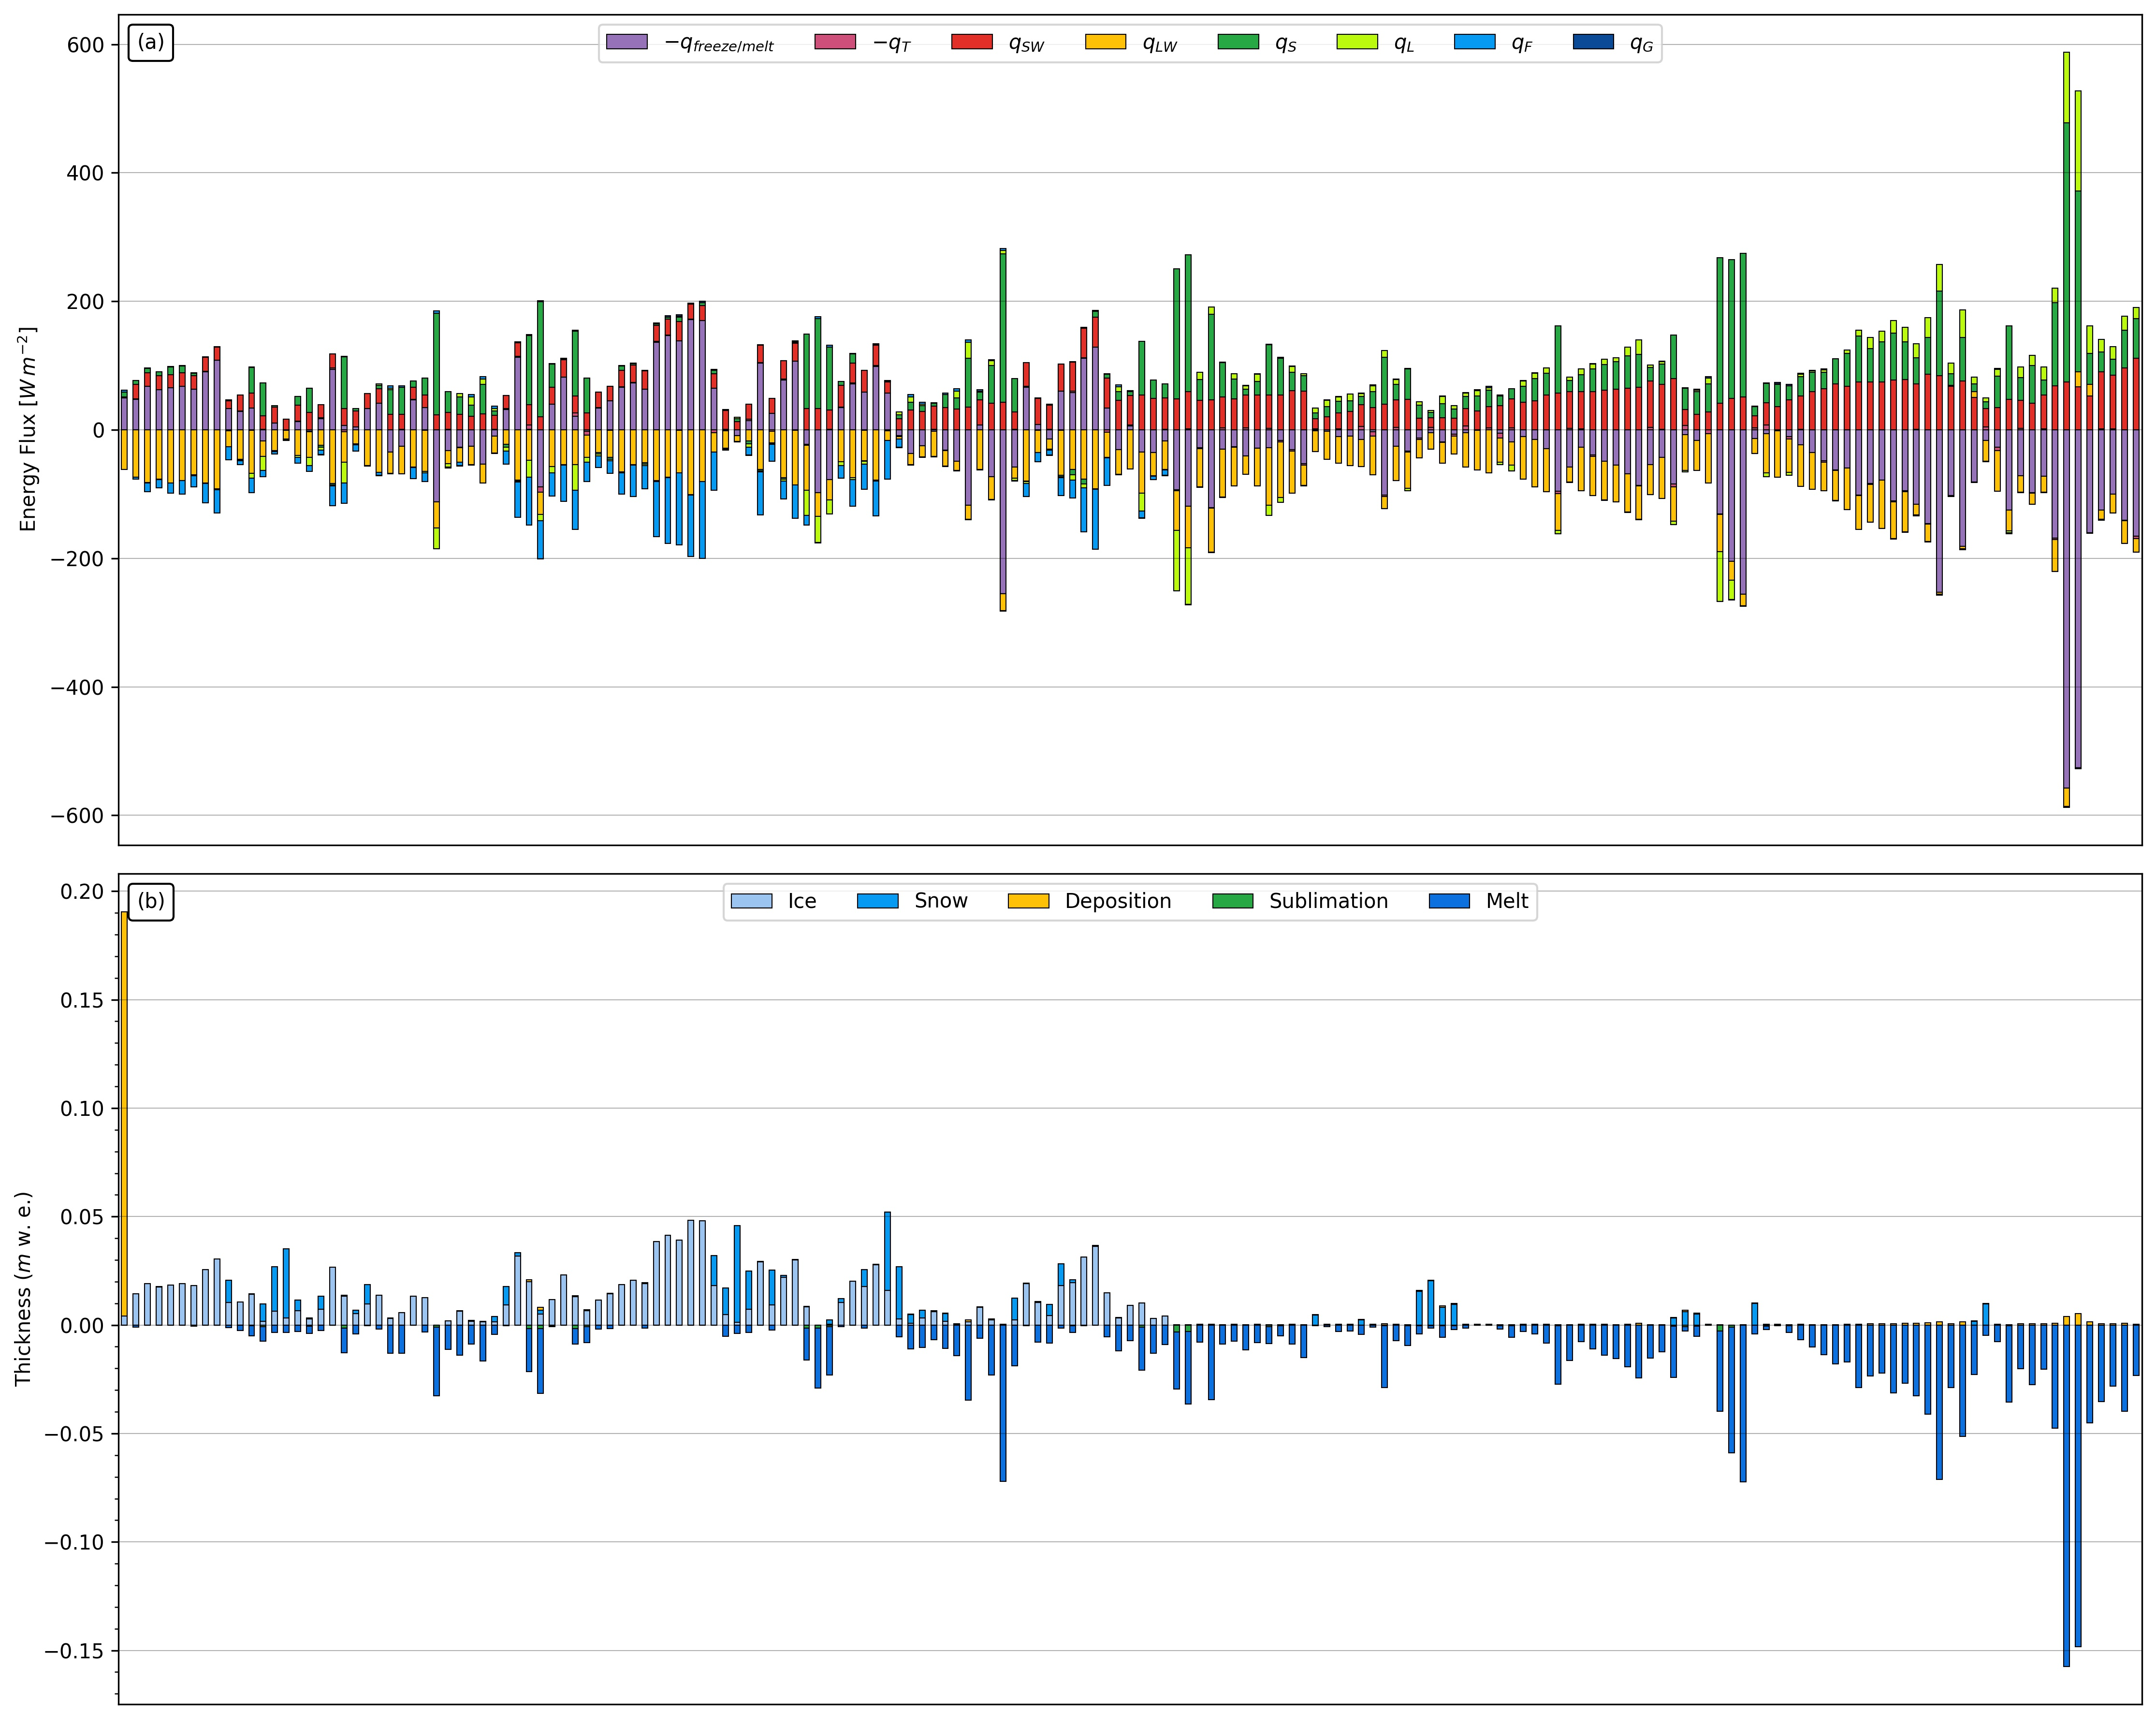
\includegraphics[width=\linewidth]{Figures/Model_Output.jpg} \end{center}
\caption{(a) Energy and (b) mass flux components of the CH21 AIR in daily time steps.  $q_{SW}$ is the
    net shortwave radiation; $q_{LW}$ is the net longwave radiation; $q_{L}$ and $q_{S}$ are the turbulent latent and
    sensible heat fluxes. $q_{F}$ represents the interactions of the fountain water with the AIR surface layer.  $q_{G}$
    quantifies the heat conduction process between the AIR surface layer and the ice body. } \label{fig:EB} \end{figure}

\subsection{Energy and mass balance calculation}

% \begin{figure} 
%     \centering
%     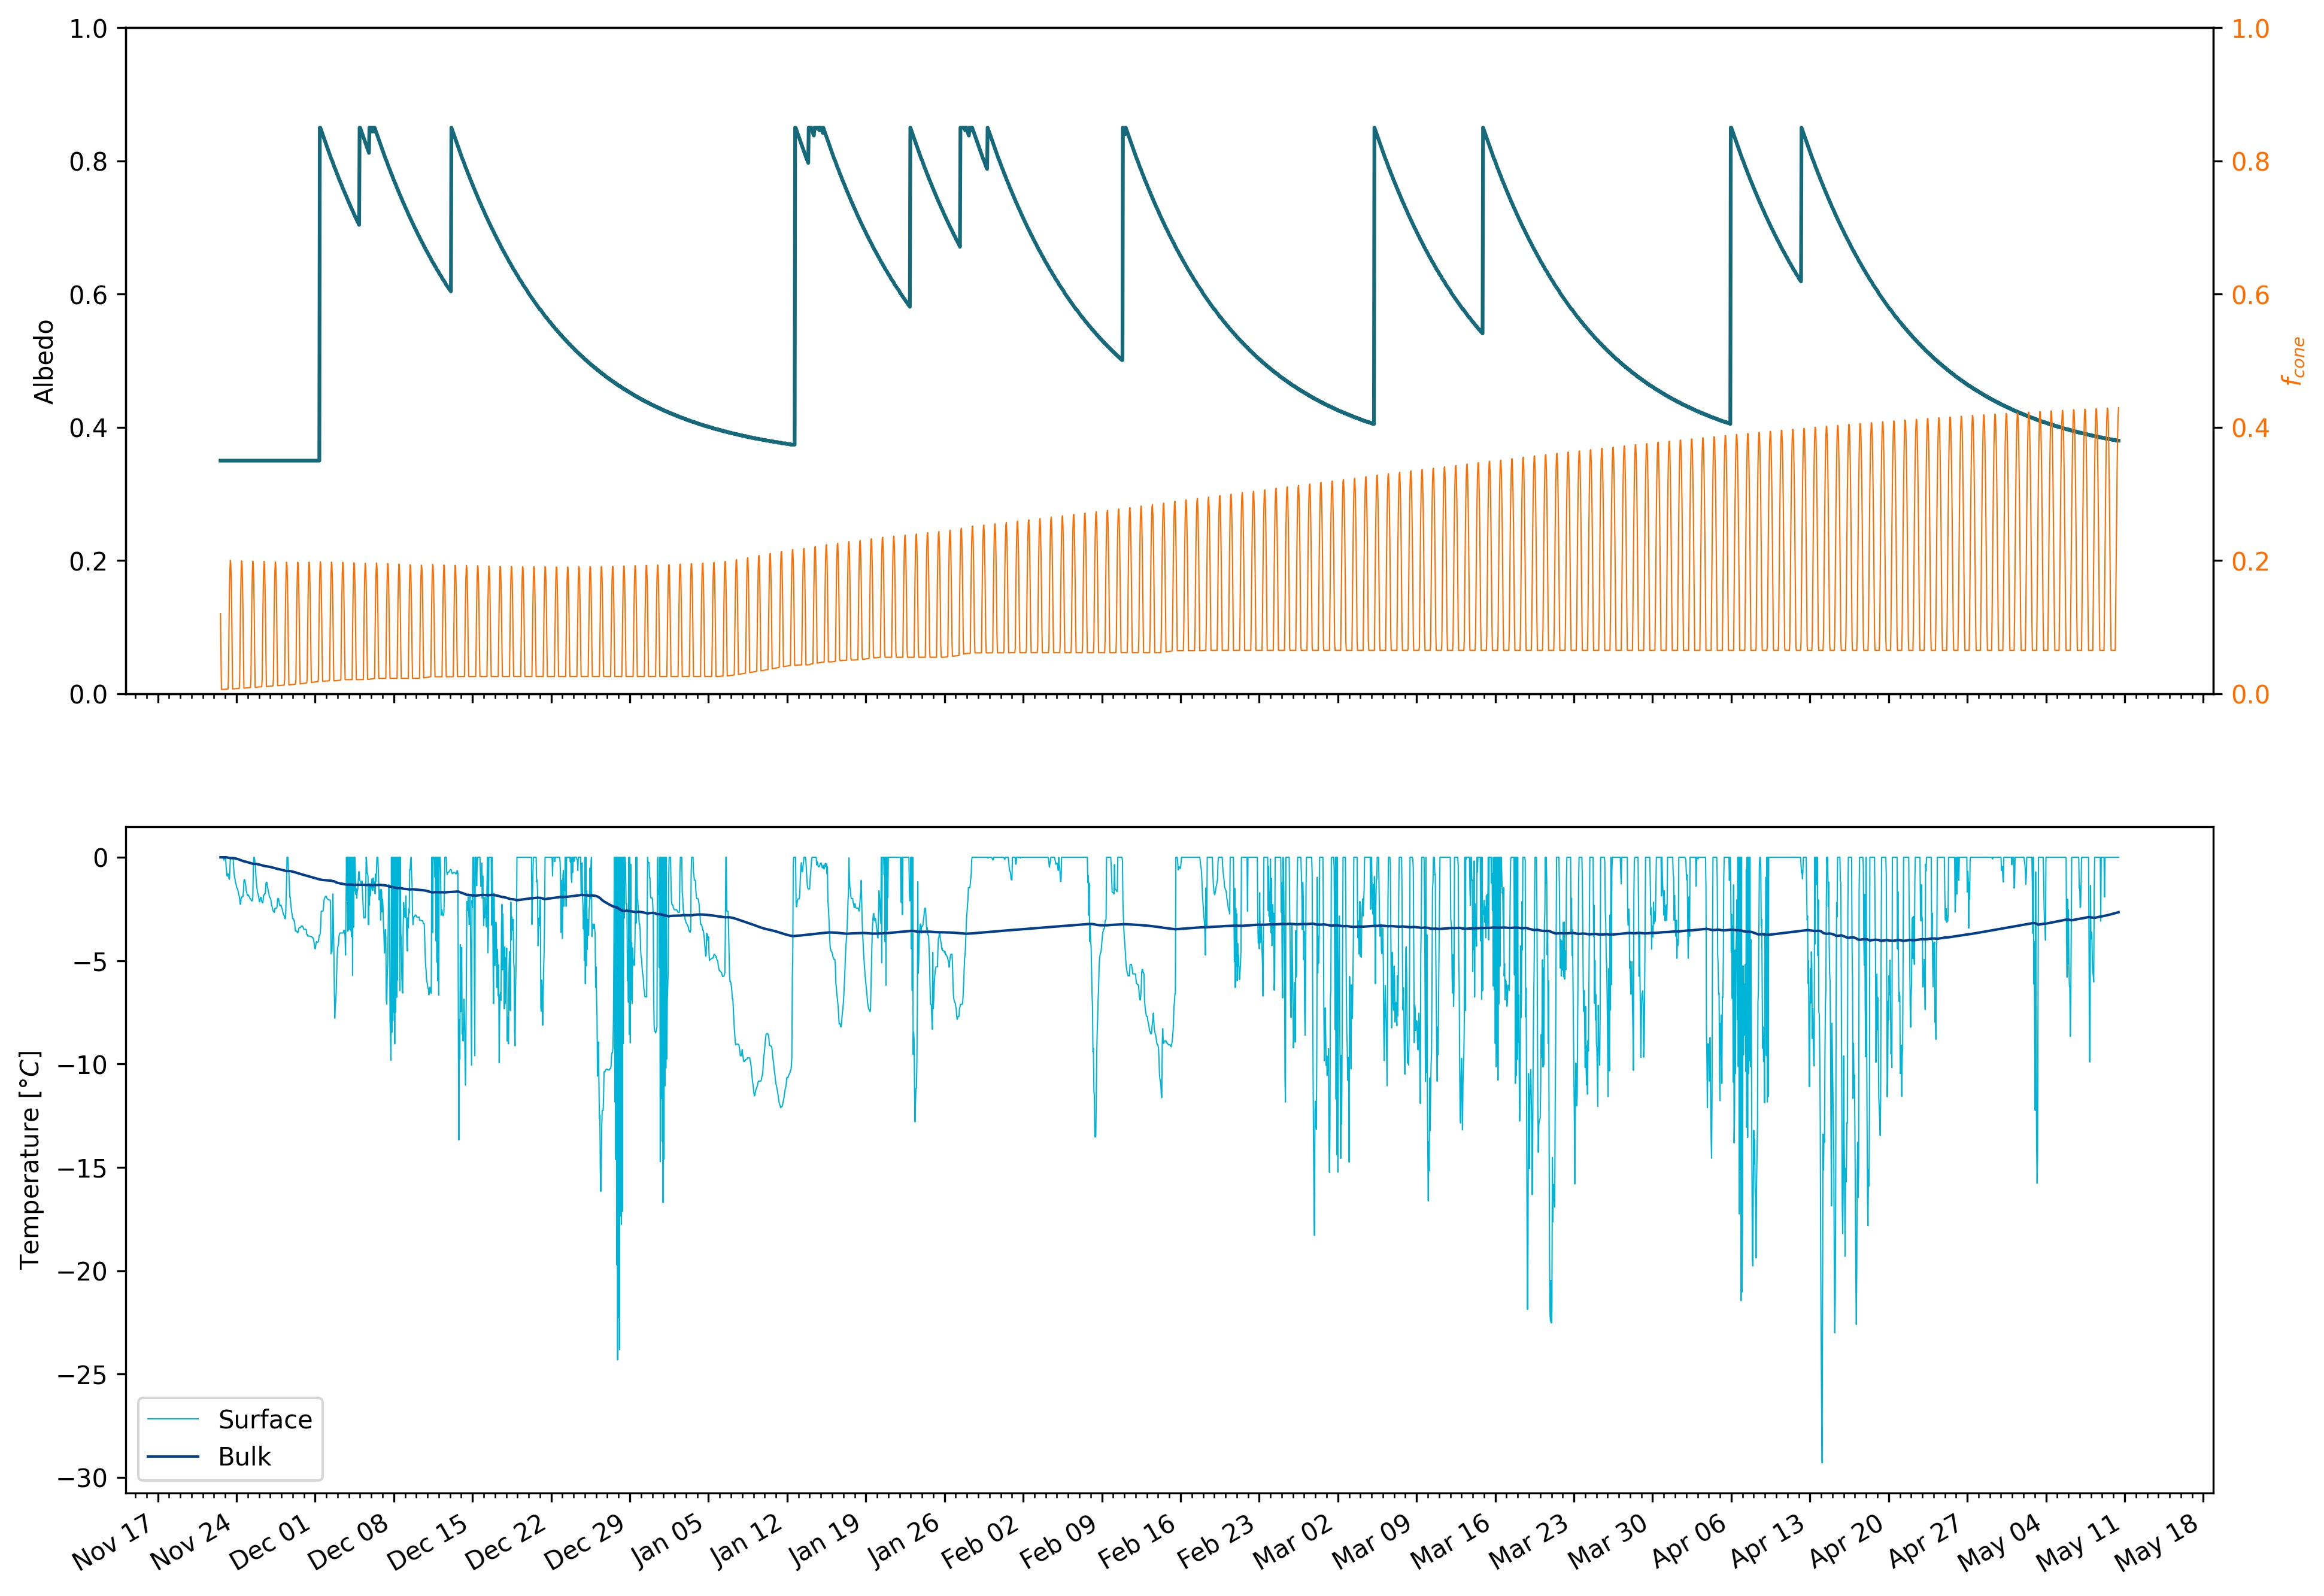
\includegraphics[width=15 cm]{Figures/albedo_temperature.jpg} 
% \caption{Some derived parameters of the model, namely, albedo and $f_{cone}$ (a), Surface and bulk temperature (b). In
%     (a), the green curve shows how snow and fountain-on events reset albedo between ice albedo and snow albedo.  The
%     decay of the snow albedo to ice albedo can also be observed. The orange curve shows how the solar radiation area
%     fraction varied diurnally with variations in the solar elevation angle. In (b), the surface temperature (light blue
%     curve) was forced to be 0 $\degree C$ during fountain activity. The corresponding bulk temperature is shown with the
%     dark blue curve.} 
% \label{fig:derived} 
% \end{figure}
  

Daily averages of some components of the energy balance are shown in Fig.  \ref{fig:EB} (b). On average during the
experiment duration, the total energy balance was almost zero. Net shortwave radiation (35 $Wm^{-2}$), sensible (41
$Wm^{-2}$) and latent heat flux (2 $Wm^{-2}$) with a mostly positive flux towards the surface of the icestupa were
compensated by the net longwave radiation (- 47 $Wm^{-2}$), the fountain water heat flux (- 13 $Wm^{-2}$) and the
freeze/melt energy (-19 $Wm^{-2}$). The contributions of other fluxes were negligible in comparison.

Net shortwave radiation is the main input to, and the most varying energy flux on the ice surface. Its variability is
controlled by the surface albedo $\alpha$ and the area fraction $f_{cone}$ which therefore represent key variables in
the energy balance (Fig. \ref{fig:derived} (b)). Although global radiation flux reached a daily maximum value of 340
$Wm^{-2}$, $q_{SW}$ only went up to 114 $Wm^{-2}$. This is caused by the fact that less than 40 \% of the direct solar
radiation influenced the Icestupa surface as shown by the area fraction $f_{cone}$ in Fig. \ref{fig:derived} (a).
Snowfall is the atmospheric variable connected most closely and proportionally to albedo.  Higher and/or more frequent
snowfall thus decreases the energy available for melt due to the corresponding increase in $\alpha$. 

$q_{LW}$ was predominantly negative indicating that this energy balance component drove the freezing of the ice
structure. Daily values of $q_{LW}$ ranged from -101 to 19 $Wm^{-2}$.  Turbulent sensible heat flux $q_{S}$ contributed
mostly to the melt of the ice structure. Daily values of $q_{S}$ ranged from -3 to 410 $Wm^{-2}$.  Daily values of the
turbulent latent heat flux $q_{L}$ ranged from -90 to 157 $Wm^{-2}$.  Since the mean of $q_{L}$ was positive, the
Icestupa gained mass cumulatively from the atmosphere due to the deposition process.  Daily values of fountain water
heat flux  ranged from -119 to 4 $Wm^{-2}$. $q_{F}$ was also a significant contributor to the freezing process like
$q_{LW}$. So the influence of the fountain on the energy balance and the freezing events was significant. The
contribution of heat flux by conduction $q_{G}$ was minimal as it only varied between -1 to 3 $Wm^{-2}$ with a
mean of 0 $Wm^{-2}$. The energy contributing to surface temperature changes ($q_{T}$) was insignificant in comparison to
the energy spent on freezing and melting ($q_{freeze/melt}$). The resulting bulk temperature and the surface temperature
are shown in Fig. \ref{fig:derived} (b).  For the total considered period, $q_{freeze/melt}$  accounted
for 30\% of overall energy turnover. The energy turnover is calculated as the sum of energy fluxes in absolute values.
$q_{LW}$ accounted for 22\%, followed by $q_{S}$ (20\%), $q_{SW}$ (16\%), $q_{L}$ (5\%), $q_{F}$ (6\%), $q_{T}$ (1\%)
and $q_{G}$ (0\%).

Fig. \ref{fig:EB} (c) represents the mass fluxes associated with these energy exchanges expressed in $m$ w.e. It shows
the ice and meltwater formed due to $q_{melt}$, snow accumulated due to precipitation, water vapour deposition and
sublimation due to $q_L$. 

% \begin{table}
% \centering
% \caption{Summary of mass balance components for the CH21 AIR at the end of the model run on $10^{th}$ May 2021.}
% \label{tab:MB}
% \begin{tabular}{@{}|ll|l|@{}}
% \toprule
% \textbf{}                                     & \textbf{Component} & \textbf{CH21} \\ \midrule
% \multicolumn{1}{|l|}{\multirow{3}{*}{\rotatebox[origin=c]{90}{Input}}}  & $M_F$              & 987,918     \\
% \multicolumn{1}{|l|}{}                        & $M_{ppt}$          & 29,533        \\
% \multicolumn{1}{|l|}{}                        & $M_{dep}$          & 4,755         \\ \midrule
% \multicolumn{1}{|l|}{\multirow{4}{*}{\rotatebox[origin=c]{90}{Output}}} & $M_{water}$        & 196,011       \\
% \multicolumn{1}{|l|}{}                        & $M_{ice}$          & 182        \\
% \multicolumn{1}{|l|}{}                        & $M_{sub}$          & 4,747         \\
% \multicolumn{1}{|l|}{}                        & $M_{runoff}$       & 821,267       \\ \bottomrule
% \end{tabular}
% \end{table}


The total water used for the Icestupa development includes contributions from the fountain (96.7\%), snowfall (2.9 \%),
deposition (0.5 \%) as shown in Table \ref{tab:MB}. Therefore, in the case of CH21 we used a water input of 1,034,328
$kg$, with a resultant storage efficiency of 19 \%.

\begin{figure} 
    \begin{center} 
    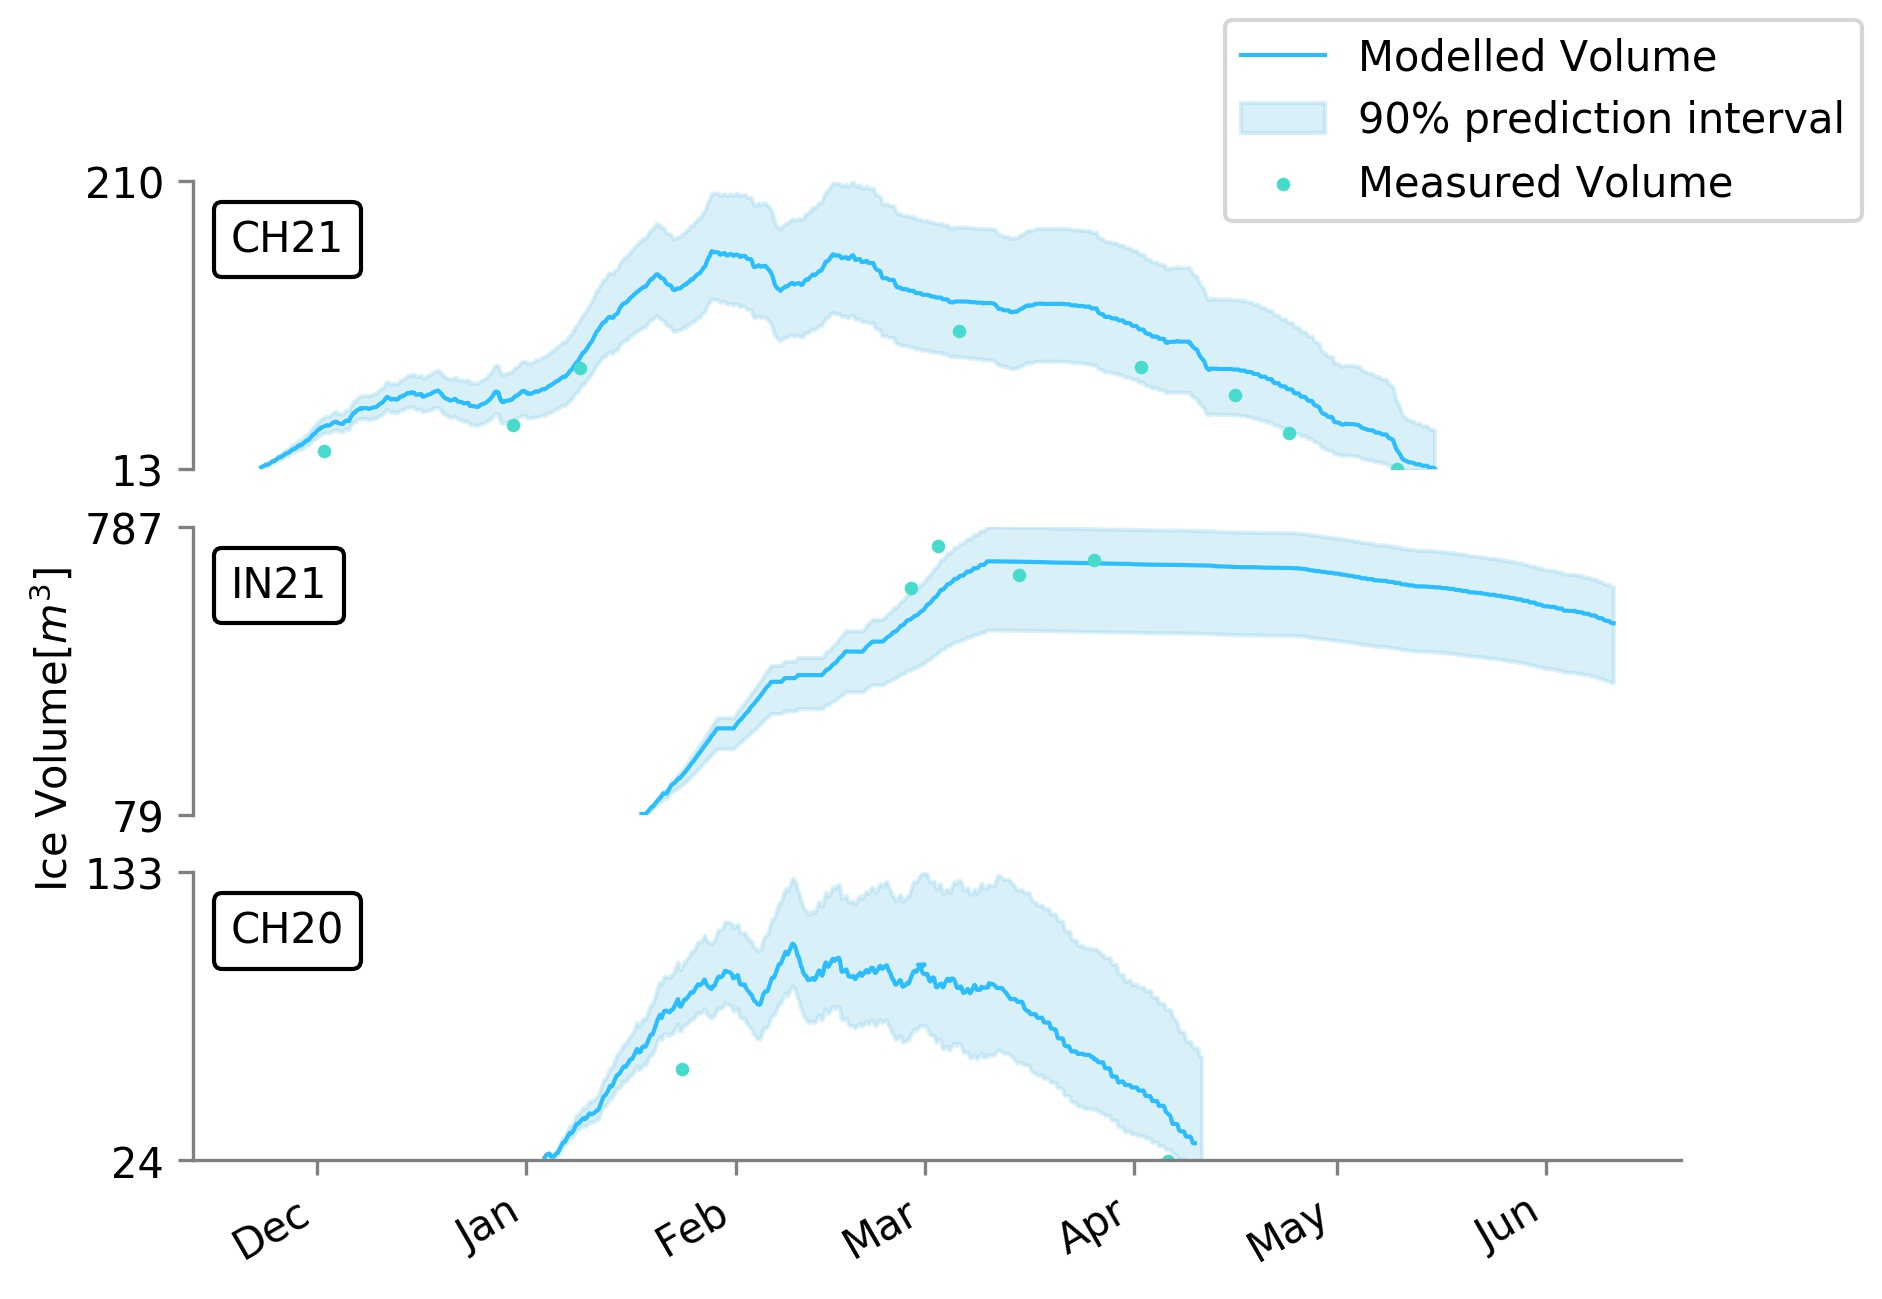
\includegraphics[width=\linewidth]{Figures/icev_results.jpg} 
\end{center}
  \caption{Modelled ice volume during the lifetime of the AIR (blue curve). Green points indicate the validation
  measurements. The prediction interval is based on the ice volume uncertainty caused by the most sensitive parameters.  } 
\label{fig:results} 
\end{figure}


\section{Model Sensitivity and Uncertainty analysis}

The icestupa model can be regarded as a function $f(x_1,x_2 \dots, x_n) = (y_1,y_2 \dots, y_m)$, where $(x_1,x_2
\dots, x_n)$ are the model parameters and $(y_1,y_2 \dots, y_m)$ are the model outputs. The influence of each
parameter on the output variables of interest were quantified and the most important physical parameters for the
subsequent uncertainty analysis were determined. The sensitivity of a parameter $x_j$ is determined by keeping all
other parameters $x_i, i \neq j$ fixed at their baseline value and varying $x_j$ within values that are physically
plausible.

A sensitivity study on the parameters (listed in Table \ref{tab:parameters}) was performed with the maximum ice
volume as the target variable. All the parameters were assumed to be independent of each other with a uniform
distribution.  This assumption ignores the auto-correlation present among the parameters associated with the albedo
parameterisation.  The range of uncertain parameters were set based on available literature values or varied $\pm$ 5\%
from the base value if no such reference was available. The uncertainty of all the site parameters were caused due to
parallax errors during manual measurement. This was quantified with a range of $\pm$ 1\% from the base value. However,
it must be kept in mind that, even though intended to be as objective as possible, the selection of a parameter range
has a subjective part that influences the results and conclusions obtained in this analysis.  The variation of the
model outputs $y_k$ is evaluated to quantify the local sensitivities $s_{j,k}$ that are defined here as the 95\% range
of the simulated outputs.

To perform the uncertainty analysis, we included only parameters that influence the maximum ice volume by at least
$0.1 m^3$. All other parameters were fixed at their baseline value.  Fig. \ref{fig:sensitivity} shows all the variance
produced by these uncertain parameters in maximum ice volume calculation. 

% It shows that $\epsilon_{ice}$ and $T_{ppt}$
% are the only parameters with a maximal sensitivity of more than 0.1 $m^3$ for the maximum ice volume estimate.
% Consequently, all other parameters were excluded from the subsequent uncertainty analysis. 
% 
% The temperature threshold below which precipitation falls as snow ($T_{ppt}$) was found to be the most sensitive
% parameter. It is used in the model to reset the albedo to snow albedo and determine snow precipitation events. The
% lower $T_{ppt}$ parameter the higher the albedo (as the Icestupa surface has a lower albedo when ice-covered than when
% snow-covered) . The variation of $T_{ppt}$ by $\pm$ $1\,\degree C$ caused maximum ice volume variation of $0.84 \pm
% 0.2 m^3$. 
% 
% Ice emissivity was also found to be a sensitive parameter. The higher the ice emissivity the larger the maximum ice
% volume as the emitted longwave radiation increases with ice emissivity. Variation of $\epsilon_{ice}$ by 5\% caused a
% maximum ice volume range from $0.98 \pm 0.1 m^3$. 
% 
In total, the sensitivity analysis required 120 simulations, and the uncertainty analysis a total of 662 simulations.

\begin{figure} 
    \begin{center} 
    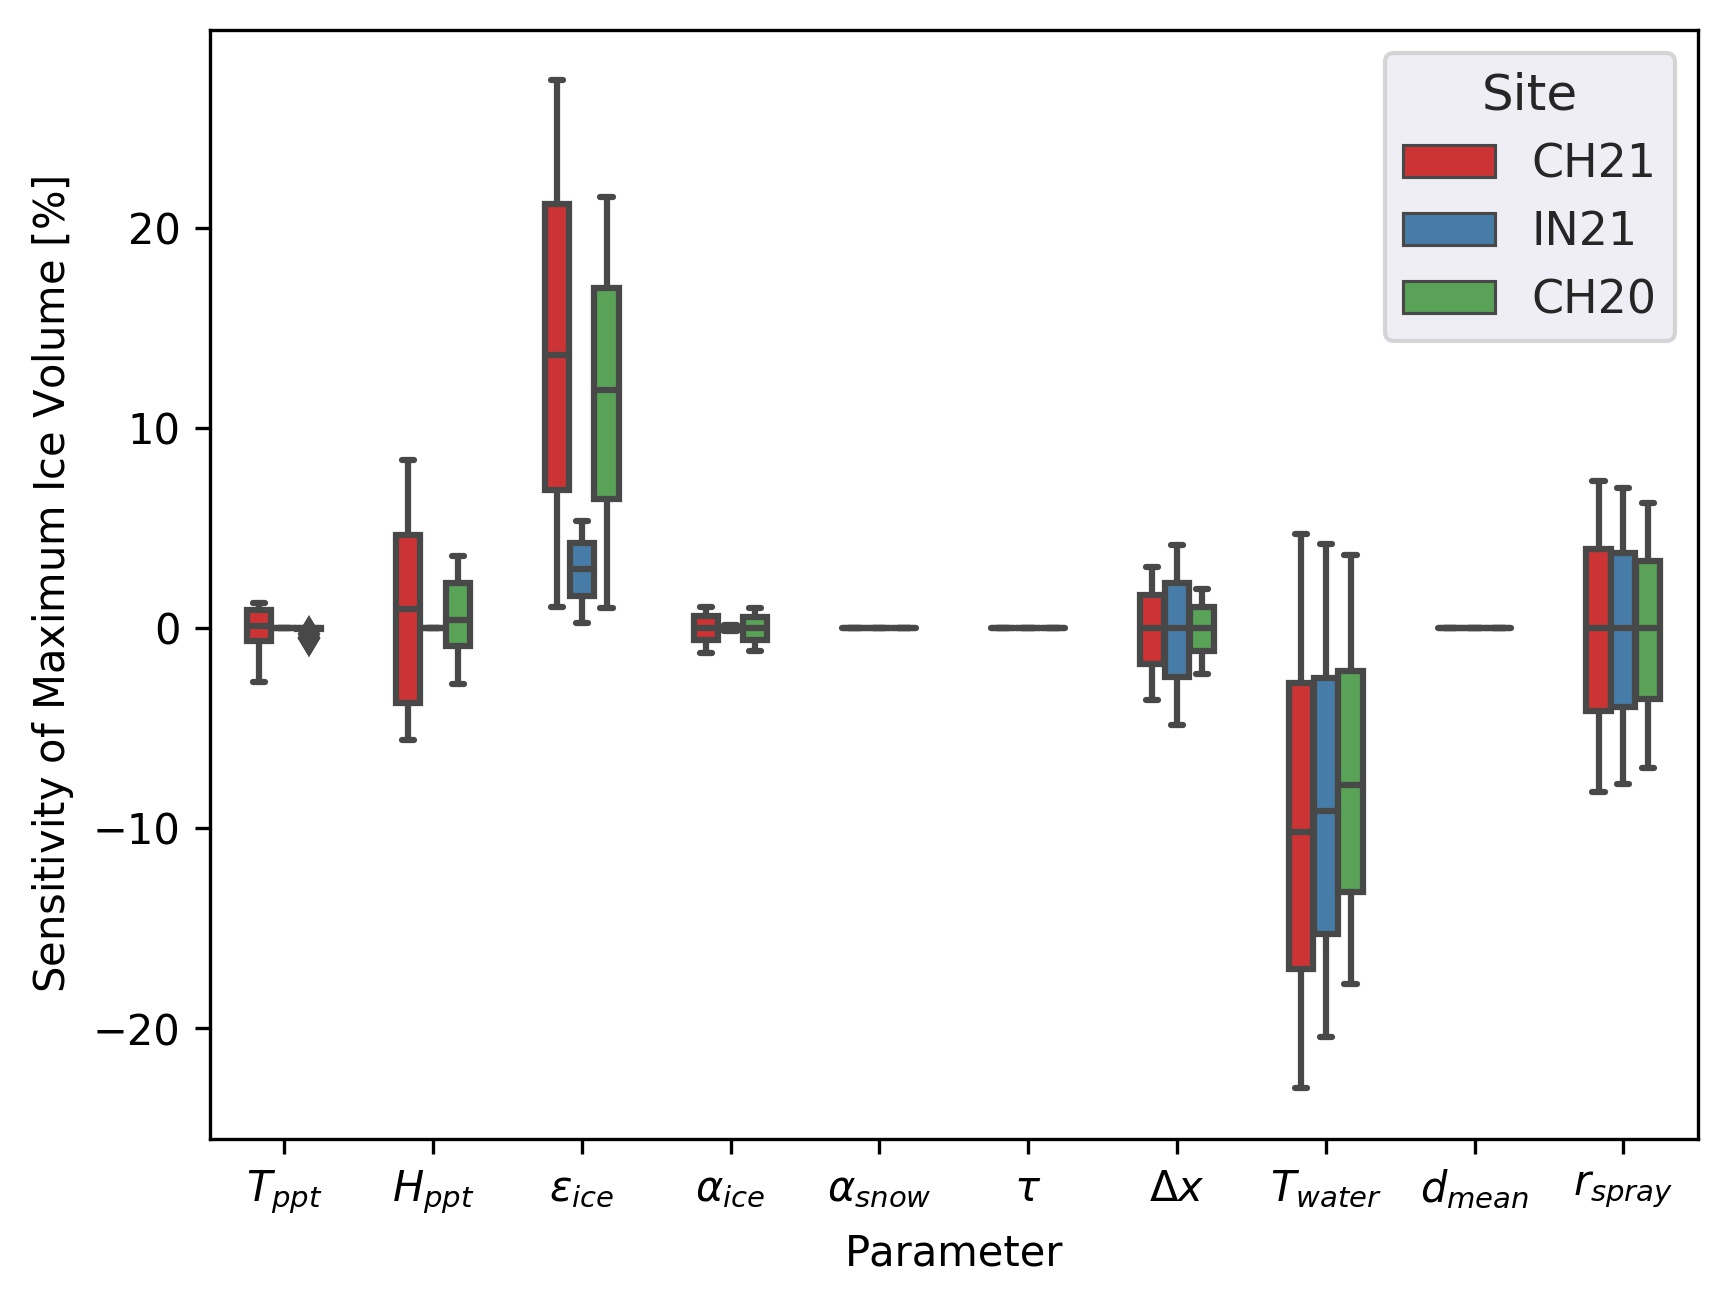
\includegraphics[width=10 cm]{Figures/sensitivities.jpg} 
\end{center}
\caption{Sensitivities of maximum ice volume to all the uncertain parameters used in the model (Table
\ref{tab:parameters}). } 
\label{fig:sensitivity} 
\end{figure}
 
\section{Discussion}
\subsection{Important assumptions}\label{section:assumptions} In the sensitivity and uncertainty analysis presented
above, we did not account for several general assumptions and parametrisation choices that may cause model errors.
Some assumptions and their potential to cause errors are discussed below.

\begin{itemize}

\item  Turbulent Sensible and Latent Heat Fluxes: The method used to calculate the turbulent heat fluxes by
  \cite{Garratt_1992} assumes that the turbulent heat fluxes are acting over a uniform planar surface to determine the
  roughness length. Since our application is on a conical surface, the distance to the ice surface is not
  uniform and well defined. Hence, $z_{ice}$ has no real physical significance here.

\item Droplet flight time loss: Water losses during the flight time of fountain droplets were neglected making all the
  fountain spray available for freezing. For the CH21 experiment, inclusion of this parameter does not influence
  results since it is already accounted for in the runoff water discharge rate which was at least $3\, l\,min^{-1}$.

\item Nucleation of droplets: Corresponding to droplet flight time, ice/snow formation is also possible before surface
  contact if nucleation occurs during flight time. For the CH21 experiment, this process will further increase
  the freeze rate and hence the storage efficiency. This process is neglected for model simplicity.
\item Shape Effects: The suppression of heat exchange between the snow/ice surface and the air adjacent to the surface
  effectively slows down snow/ice ablation in spring and promotes the stagnation of the cold air within topographical
  depressions \citep{Fujita_2010}. The quantitative contribution of the atmospheric decoupling over melting snow/ice
  for the total mass and energy balance is ignored in the model.

\end{itemize}

\section{Conclusions} 
We outlined a methodology for estimating ice, liquid water, water vapour and runoff quantities produced during the
construction of an AIR using measurements of fountain spray rate, air temperature, radiation, humidity, pressure,
wind and cloudiness at four different study sites. The comparison with all the validation measurements at two different
dates during the experiment led to satisfying results as shown in Table \ref{tab:results}.

% According to the model, the CH19 AIR achieved a storage quantity of 1005 litres of water with a storage
% duration of 65 days. However, the corresponding storage efficiency of 6 \% was very low for a water input of 18,560
% litres. These estimates were most sensitive to the temperature threshold that determined precipitation phase and ice
% emissivity parameters which created an uncertainty of $0.2 m^3$ in the maximum ice volume calculated.  This is
% to be expected as net longwave radiation and net shortwave radiation together accounted for around 65 \% of the overall
% energy turnover.

The model results support the hypothesis that there could be considerable water loss during the formation of AIR
particularly due to excessive fountain spray. Further experiments at different locations with different fountains are
required to better understand the influence of construction decisions on the results. 

\begin{table}
\centering
\caption{AIR Results}
\label{tab:results}
\begin{tabular}{@{}|l|l|l|l|l|@{}}
\toprule
\textbf{AIR}   & \textbf{IN21} & \textbf{CH21} & \textbf{CH20} & \textbf{CH19} \\ \midrule
Max Ice Volume [$m^3$] & 703             & 156             & 107             & 1             \\ \midrule
Storage Efficiency [$\%$] & 18             & 19             & 14             & 3             \\ \midrule
Storage Duration [$days$] & ?             & 169             & 93             & 45             \\ \bottomrule
Validation RMSE [$m^3$] & 59             & 13             & 25             & 0.2             \\ \bottomrule
\end{tabular}
\end{table}


\section{Appendix}

\subsection{Ladakh Icestupa 2014/15} \label{section:ladakhloss} 
A 20 $m$ tall Icestupa \citep{iceheight} was built in Phyang village, Ladakh at an altitude of 3500 $m$ a.s.l. Assuming
a conical shape with a diameter of 20 $m$, the corresponding volume of this Icestupa becomes 2093 $m^3$ or 1,920 $m^3$
w.e. The fountain sprayed water at a rate of $210\, l\,min^{-1}$ \citep{waterinput} from $21^{st}$ January
\citep{waterstart} to at least until $5^{th}$ March 2015 \citep{waterend} (around 43 nights). Assuming fountain spray
was active for 8 hours each night, we estimate water consumption to be around 4,334 $m^3$. Thus, during the
construction/freezing period of the Icestupa, roughly 56 \% of the water provided was wasted. The actual water loss is
bound to be much higher due to further vapour losses during the melting period. This Icestupa completely melted away on
$6^{th}$ July 2015 \citep{iceends}. Therefore, the storage duration was 166 days or roughly 5 months. 

% \subsection{CH19 AIR}\label{section:CH19}
% The CH19 AIR in the Schwarzsee region lies at 967 $m$ a.s.l.. In the winter (Oct-Apr), mean daily maximum
% and minimum air temperatures vary between -4 and 14 $\degree C$. Clear skies are rare, averaging around 7 days, and
% precipitation amounts average 155 mm per month during winter \citep{eispalast}. The site was situated adjacent to a
% stream resulting in high humidity values across the study period. Within the EP site, an enclosure with a 1.8\,$m$
% radius was constructed for the experiment. An automatic weather station (AWS) was adjacent to the wooden
% boundary as shown in Fig. \ref{fig:site}. The fountain used for spraying water had a nozzle diameter of 5\,$mm$ and a
% height of 1.35\,$m$, and was placed in the centre of the wooden enclosure. The water was transferred from a spring
% water source at 1267 $m$ a.s.l. by pipeline and flowed via a flowmeter and an air escape valve to the nozzle, where it
% was sprinkled with a spray radius of around 1.7\,$m$. The air escape valve was installed to avoid errors in the flow
% measurements due to air bubbles. In addition, a webcam guaranteed a continuous survey of the site during the
% construction of the Icestupa. 
% 
% \begin{figure} 
%     \centering 
%     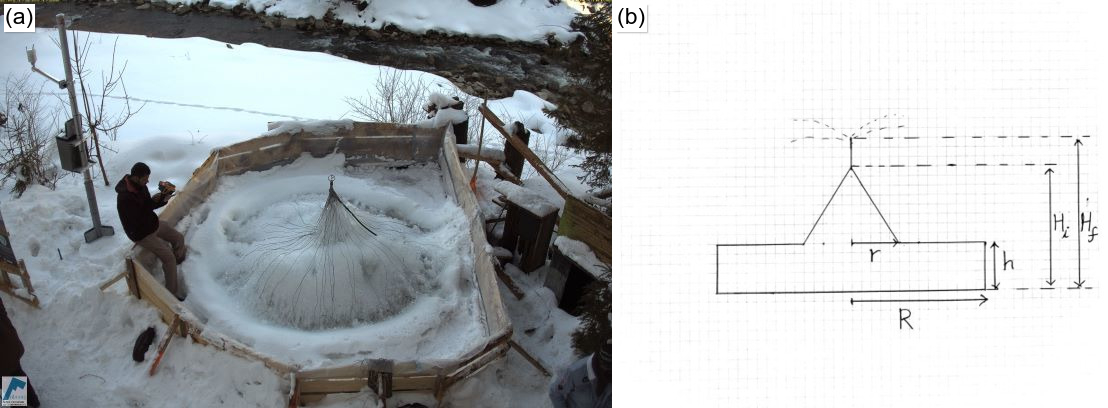
\includegraphics[width=15cm]{./Figures/Figure_2.jpg}
% \caption{(a) The ice structure during the first validation measurement as seen on the webcam image of
%   $14^{th}$ Feb. (b) The corresponding cross section of the EP ice structure with the field estimates of $r, R,
%   h, H_i, H_f$ used to determine the Icestupa volume is shown on the right.} 
%   \label{fig:CH19site} 
%   \end{figure}
% 
% \subsubsection{Weather data}
% Precipitation data was derived from the Plaffeien AWS \citep{meteoswiss} located 8.8 km away from the measurement site
% at an altitude of 1042 $m$ a.s.l.  We recognised during our data analysis that, except precipitation, all the other
% meteorological variables of the EP site correlated much better with the ERA5 dataset than the nearby Plaffeien AWS
% dataset. The $2\,m$ temperature parameter correlated with air temperature ($r^2 =0.9 $), surface pressure parameter
% correlated with air pressure ($r^2 = 1$) and 10m wind speed parameter (derived from horizontal and vertical components)
% correlated with wind speed ($r^2 =0.6 $) .
% 
% Due to a power failure, all data from the EP AWS was lost from $27^{th}$ February 15:20 2019 to $2^{nd}$ March 15:00
% 2019 (equivalent to around 7\% of the measurement period). During heavy snowfall events, the ultrasonic wind sensor was
% blocked and recorded zero values. ERA5 was used to fill such errors and data gaps .
% 
% The ERA5 grid point chosen (Latitude 46° 38' 24" N, Longitude 7° 14' 24" E) for the EP site was around 9 km away from
% the actual site. Near-surface humidity is not provided directly in ERA5 dataset, but from near-surface ($2\,m$ from the
% surface) temperature ($T_{ERA5}$) and dew point temperature ($Tw_{ERA5}$) the relative humidity ($RH$) at $2\,m$  was
% calculated as: 
% 
% \begin{equation} RH = 100 \cdot
%     \frac{e_{sat}(Tw_{ERA5})}{e_{sat}(T_{ERA5})} \end{equation} 
% 
% where the saturation vapour pressure function $e_{sat}$ is expressed with the Teten's formula \citep{Tetens}:
% \begin{equation} e_{sat}(T)= a_1 \cdot e^{(a_3 \cdot \frac{T}{(T+273.16-a_4)})} \end{equation} with T in $\degree C$ and
% the parameters set for saturation over water ($a_1$ = 611.21 Pa, $a_3$ = 17.502 and $a_4$= 32.19 K) according to
% \cite{Buck_1981}.    
% 
% All the ERA5 variables were therefore fitted with the EP dataset via linear regressions.  With the modified ERA5
% dataset, we were also able to further extend the EP dataset and allow the model to run beyond $18^{th}$ March 2019.
% Precipitation was filled as null values beyond $18^{th}$ March 2019.
% 
% \subsubsection{Fountain spray radius of CH19 AIR} \label{section:sprayCH19} 
% This fountain spray radius is determined by modelling the projectile motion of the water droplets. Using mass
% conservation, the droplet speed $v_F$ can be determined from the spray rate $d_F$ and the diameter $dia_F$ of the nozzle
% as follows:
% 
% \begin{equation} v_F = \frac{d_F}{\pi \cdot dia_F^2/4} \end{equation}
% 
% Afterwards, we assume that the water droplets move with an air friction free projectile motion from the fountain
% nozzle with a height $h_F$ to the ice/ground surface. The resulting spray radius $r_F$ was then determined from the
% projectile motion equation as follows:
% 
% \begin{equation} r_F = \frac{v_F \cdot cos\theta_F (v_F \cdot sin\theta_F + \sqrt{(v_F \cdot sin\theta_F)^{2} + 2
% \cdot g \cdot h_F})}{g} \end{equation}
% 
% where $g = 9.8\, m s^{-2}$ is the acceleration due to gravity and $\theta_F$ = 45 $\degree$ is the angle of launch.
% 
% \subsubsection{CH19 Field Measurements for validation} \label{section:validation} 
% The volume was determined by decomposing the ice structure into a cylinder (length $2R$ and height $h$) and a
% cone (radius $r$ and height $(H_i-h)$) through the following equation: 
% \begin{equation} V = \pi \cdot R^2 \cdot h + 1/3 \cdot \pi \cdot r^2 \cdot (H_i-h) \end{equation}
% 
% Manual measurements were performed at the end of the freezing period on $14^{th}$ February 16:00 2019 (only one more
% fountain run was possible after this date) to estimate $r, R, h, H_i, H_f$ (see Fig. \ref{fig:site} for the different
% geometry components):
% 
% $$ 0.55\leq r\leq 1 m\textit{ ; }1.1\leq R\leq 1.2 m\textit{ ; }0.1\leq h\leq 0.2 m\textit{ ; }0.6\leq
% H_i\leq 0.8 m\textit{ ; }1.3\leq H_f\leq 1.4 m  $$
% 
% The ranges of the variables show the variance of the Icestupa's dimensions across different compass orientations.
% Correspondingly, the volume range estimated for the first validation point was 0.857 $\pm$ 0.186 $m^{3}$ on $14^{th}$
% February 16:00 2019.
% 
% The second validation point corresponds to the end of the melting process on $10^{th}$ March 18:00 2019.  Based on the
% webcam imagery and manual measurement, a thin layer of ice with an observed thickness between 0.01 to 0.06 m could be
% quantified. This results in the volume range for the second validation to be 0.13 $\pm$ 0.09 $m^{3}$ on $11^{th}$ March
% 2019 
% 
% In reality, the EP ice structure was more cylindrical until a height of 0.2\,$m$ and conical afterwards until a
% height of 0.6\,$m$ with a radius of 1.18\,$m$. However, we assume a conical shape of this ice structure in order to
% apply the modelling strategy described below.

% \subsubsection{CH21 and CH20 Surface temperature corrections} \label{section:thermalcam} 
% We discarded some thermal camera temperature measurements due to the following reasons:
% \begin{itemize} 
%     \item Snowfall/fog: Whenever there was snow or thick fog, the thermal image was corrupted. Refer image Jan14 1900 and
% Jan3 800. We used the standard deviation of the pixel temperature to identify these events and remove them from the
% validation dataset. 
% 
% \item Strong sunlight: Usually at noon, especially in end of Feb and March, we observed that ice temperature values were
%     above zero C. We found that again the thermal cam images were corrupted as seen in Mar6 1300. So we removed all
%     temperature values above 0 C.  
% 
% \item Then there were some images that were completely blue and looked corrupted.  We cannot identify the cause here but
%     I filtered them out using the mean of all temperature pixels.
% 
% \end{itemize} 

% The IN21 AIR was constructed as part of the Icestupa Competition in Gangles, Ladakh, India. It was constructed adjacent
% to another AIR and merged with it. To initiate the ice formation process, a dome of 2\,$m$ radius was constructed and
% the fountain pipeline was erected at the center using a tripod. Fountain operation was interrupted only due to pipeline
% freezing events. The fountain height varied between 5 to 9\,$m$.
% 
% The CH19 AIR was constructed by the Eispalast in Schwarzsee, Switzerland. It was contained inside a wooden boundary
% adjacent to a stream. Fountain operation was guided by temperature conditions.  The water spray of the fountain was
% initially adjusted so that most of the water droplets land within the wooden boundary zone. The ice formation was guided
% by adding a metal framework at the ice structure base after the first night of operation.  Several cotton threads were
% tied between the ice structure base and fountain pole for accelerating and further guiding the ice formation process. 

% \section*{Conflict of Interest Statement} The authors declare that the research was conducted in the absence of any
% commercial or financial relationships that could be construed as a potential conflict of interest.
% 
% \section*{Author Contributions} SB wrote the initial version of the manuscript. MH, ML, SW, JO, and FK commented on
% the initial manuscript and helped improve it. SB developed the methodology with inputs from MH. SB performed the
% analysis with support from MH and ML. SB and MH participated in the fieldwork.
% 
% \section*{Funding} This work was supported and funded by the University of Fribourg and by the Swiss Government
% Excellence Scholarship (SB).
% 
% \section*{Acknowledgments} We thank Mr. Adolf Kaeser and Mr. Flavio Catillaz at Eispalast Schwarzsee for their active
% participation in the fieldwork. We would also like to thank Digmesa AG for subsidising their flowmeter used in the
% experiment. We would particularly like to thank the editor Prof. Thomas Schuler and 2 anonymous reviewers who gave us
% important inputs to improve the paper. We also thank Prof. Christian Hauck, Prof. Nanna B. Karlsson and Dr. Andrew
% Tedstone for valuable suggestions that improved the manuscript.
% 
% \section*{Data Availability Statement} The data and code used to produce results and figures will be published at a
% later stage and can, until then, be obtained from the authors upon request.

\bibliographystyle{frontiersinSCNS_ENG_HUMS} \bibliography{references}

\end{document}
